\documentclass[9pt,twocolumn,a4paper]{extarticle}

\usepackage{amsmath}
\usepackage{fontspec}
\usepackage{unicode-math}
\setmainfont{CharisSIL-Regular.ttf}[BoldFont=CharisSIL-Bold.ttf,ItalicFont=CharisSIL-Italic.ttf,BoldItalicFont=CharisSIL-BoldItalic.ttf]
\setmathfont{STIXTwoMath-Regular.otf}
\setmonofont{consola.ttf}[BoldFont=consolab.ttf,ItalicFont=consolai.ttf,Scale=0.9]
\usepackage[top=1.5cm,bottom=2.3cm,left=1.35cm,right=1.35cm,columnsep=0.75cm,footskip=0.9cm,headsep=0.45cm]{geometry}
\usepackage{graphicx}
\usepackage{booktabs}
\usepackage{array}
\usepackage{xcolor}
\usepackage{titlesec}
\usepackage{caption}
\usepackage{float}
\usepackage{tikz}
\usetikzlibrary{arrows.meta,positioning}
\usepackage{fancyhdr}
\usepackage{microtype}

\definecolor{linkblue}{RGB}{0,106,150}
\definecolor{bannergray}{RGB}{229,229,229}
\usepackage[colorlinks=true,linkcolor=linkblue,citecolor=linkblue,urlcolor=linkblue]{hyperref}

\tikzset{
  pbox/.style={draw=linkblue,thick,rounded corners=2pt,fill=linkblue!8,align=center,
               minimum height=8mm,text width=15mm,font=\scriptsize},
  pmine/.style={pbox,fill=linkblue!25,very thick},
  parr/.style={-{Stealth[length=2mm]},thick}}

\titleformat{\section}{\large\bfseries\color{linkblue}}{Chương \thesection.}{0.5em}{}
\titleformat{\subsection}{\normalsize\bfseries}{\thesubsection.}{0.5em}{}
\titlespacing*{\section}{0pt}{12pt}{5pt}
\titlespacing*{\subsection}{0pt}{7pt}{2pt}
\setlength{\parskip}{1.5pt}
\setlength{\parindent}{0pt}
\setlength{\arraycolsep}{2pt}
\setlength{\abovedisplayskip}{4pt}
\setlength{\belowdisplayskip}{4pt}
\renewcommand{\figurename}{Hình}
\renewcommand{\tablename}{Bảng}
\renewcommand{\refname}{Tài liệu tham khảo}
\captionsetup{font={footnotesize},labelfont=bf,labelsep=period,justification=justified,singlelinecheck=false,skip=3pt}
\captionsetup[table]{position=top}
\emergencystretch=3em
\setlength{\textfloatsep}{9pt plus 2pt minus 2pt}
\setlength{\floatsep}{7pt plus 2pt minus 2pt}
\setlength{\intextsep}{7pt plus 2pt minus 2pt}
\linespread{1.02}
\raggedbottom

\newcommand{\code}[1]{\texttt{#1}}
\newcommand{\spaced}[1]{\textls[160]{#1}}
% Tiêu đề một cấu trúc dữ liệu: tên bên trái, lớp Java bên phải
\newcommand{\dsa}[2]{\subsection[#1]{#1\hfill{\normalfont\footnotesize\code{#2}}}}
% Ba nhãn cố định cho mỗi mục
\newcommand{\vande}{\textcolor{linkblue}{\textbf{Vấn đề.}}~}
\newcommand{\cachgiai}{\textcolor{linkblue}{\textbf{Cách giải.}}~}
\newcommand{\dpt}{\textcolor{linkblue}{\textbf{Độ phức tạp.}}~}

\newcommand{\runauthor}{\textit{L.\,A.\ Kiet}}
\newcommand{\runtitle}{\textit{Cấu trúc dữ liệu và giải thuật trong CocCoc Plus}}
\pagestyle{fancy}
\fancyhf{}
\renewcommand{\headrulewidth}{0pt}
\fancyhead[L]{\footnotesize\runauthor}
\fancyhead[R]{\footnotesize\runtitle}
\fancyfoot[C]{\footnotesize\thepage}
\fancypagestyle{first}{\fancyhf{}\renewcommand{\headrulewidth}{0pt}}

\makeatletter
\renewcommand\@biblabel[1]{\textcolor{linkblue}{[#1]}}
\makeatother

\newcommand{\cu}{\textcolor{linkblue}{\textbf{Cách cũ.}}~}
\newcommand{\vidu}{\textcolor{linkblue}{\textbf{Ví dụ.}}~}

\begin{document}
\thispagestyle{first}

\twocolumn[{%
\begin{@twocolumnfalse}
\vspace{-0.3cm}
\begin{center}\small\color{linkblue}Cấu trúc dữ liệu và giải thuật, tài liệu kiến thức đi kèm đồ án (2026)\end{center}
\vspace{-0.1cm}
\noindent\rule{\textwidth}{0.5pt}\\[-2pt]
\noindent\colorbox{bannergray}{\parbox{\dimexpr\textwidth-2\fboxsep}{\centering\vspace{3pt}
  {\small Môn học: Cấu trúc dữ liệu và giải thuật \;$\cdot$\; Trường Đại học Quốc tế, ĐHQG-HCM}\\[7pt]
  {\Large Kiến thức nền cho CocCoc Plus}\vspace{4pt}}}\\[-1pt]
\noindent\rule{\textwidth}{2.2pt}

\vspace{0.55cm}
{\fontsize{16.5}{20}\selectfont Cấu trúc dữ liệu và giải thuật trong máy tìm kiếm CocCoc Plus:\\mỗi cấu trúc giải quyết vấn đề gì\par}
\vspace{0.4cm}
{\large Lê Anh Kiệt\textsuperscript{\,a}\par}
\vspace{0.2cm}
{\scriptsize\textsuperscript{a}\,\textit{Trường Đại học Quốc tế, Đại học Quốc gia TP. Hồ Chí Minh, Việt Nam} \quad MSSV: ITCSIU24047\par}
\vspace{0.3cm}
\noindent\rule{\textwidth}{0.4pt}
\vspace{0.25cm}

\noindent\begin{minipage}[t]{0.255\textwidth}
{\footnotesize\spaced{T Ừ \ \ K H Ó A}\par}
\vspace{2pt}\noindent\rule{\linewidth}{0.4pt}\par\vspace{3pt}
{\scriptsize
Hàng đợi, min-heap, Bloom filter\\
Bảng băm, LRU cache\\
Trie, quy hoạch động\\
Chỉ mục đảo, VByte\\
Hai con trỏ, galloping search\\
Ma trận thưa CSR, cửa sổ trượt\par}
\end{minipage}\hfill
\begin{minipage}[t]{0.715\textwidth}
{\footnotesize\spaced{T Ó M \ \ T Ắ T}\par}
\vspace{2pt}\noindent\rule{\linewidth}{0.4pt}\par\vspace{3pt}
{\scriptsize\setlength{\parindent}{0pt}\linespread{1.08}\selectfont
Tài liệu liệt kê các cấu trúc dữ liệu và giải thuật mà CocCoc Plus tự cài đặt, chia theo ba khối. Chương~1 (Crawler) dùng hàng đợi, min-heap, Bloom filter, bảng băm và LRU cache. Chương~2 (Chỉ mục và truy vấn) dùng trie, quy hoạch động, chỉ mục đảo nén VByte, hai con trỏ và galloping search. Chương~3 (Xếp hạng) dùng ma trận thưa CSR cho PageRank, min-heap lấy top-$K$ và cửa sổ trượt tạo đoạn trích. Mỗi mục nêu vấn đề trong đồ án, cách cũ hỏng ở đâu, cách giải, một ví dụ số và độ phức tạp.\par}
\end{minipage}

\vspace{0.25cm}
\noindent\rule{\textwidth}{0.4pt}
\vspace{0.35cm}
\end{@twocolumnfalse}
}]

\begin{figure}[H]
\centering
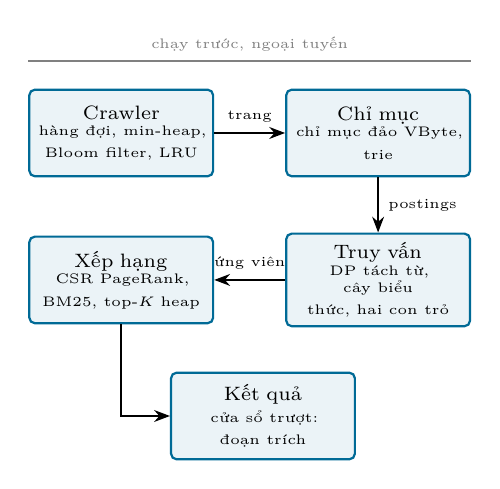
\begin{tikzpicture}[node distance=9mm,
  b/.style={pbox,text width=21mm,minimum height=11mm,font=\scriptsize}]
  \node[b] (crawl) {Crawler\\\tiny hàng đợi, min-heap,\\\tiny Bloom filter, LRU};
  \node[b,right=of crawl] (index) {Chỉ mục\\\tiny chỉ mục đảo VByte,\\\tiny trie};
  \node[b,below=7mm of index] (query) {Truy vấn\\\tiny DP tách từ, cây biểu\\\tiny thức, hai con trỏ};
  \node[pmine,b,left=of query] (rank) {Xếp hạng\\\tiny CSR PageRank,\\\tiny BM25, top-$K$ heap};
  \node[b,below=6mm of rank,xshift=18mm] (out) {Kết quả\\\tiny cửa sổ trượt: đoạn trích};
  \draw[parr] (crawl) -- node[above,font=\tiny]{trang} (index);
  \draw[parr] (index) -- node[right,font=\tiny]{postings} (query);
  \draw[parr] (query) -- node[above,font=\tiny]{ứng viên} (rank);
  \draw[parr] (rank.south) |- (out.west);
  \draw[gray] ([yshift=3.5mm]crawl.north west) -- node[above,font=\tiny,gray]{chạy trước, ngoại tuyến} ([yshift=3.5mm]index.north east);
\end{tikzpicture}
\caption{Năm bước của máy tìm kiếm và cấu trúc dữ liệu chính ở mỗi bước. Hai bước trên chạy trước, ba bước dưới chạy cho mỗi truy vấn, nên mỗi truy vấn chỉ chạm vào một phần nhỏ của kho.}
\label{fig:pipeline}
\end{figure}

\begin{table}[H]
\centering\scriptsize
\renewcommand{\arraystretch}{1.1}
\begin{tabular}{@{}p{10mm}p{66mm}@{}}
\toprule
Bước & Ví dụ xuyên suốt: truy vấn ``nhà hàng xóm'' \\
\midrule
Crawler & 3 trang: $d_1$ ``nhà hàng xóm Hải'', $d_2$ ``nhà hàng ngon quận 1'', $d_3$ ``hàng xóm mới chuyển nhà'' \\
Chỉ mục & nhà $\to\{1,2,3\}$; nhà hàng $\to\{1,2\}$; hàng xóm $\to\{1,3\}$ \\
Truy vấn & hai cách tách từ: ``nhà hàng'' + ``xóm'' hoặc ``nhà'' + ``hàng xóm''; giao postings được $\{1,3\}$ \\
Xếp hạng & điểm BM25 và PageRank, top-2: $d_1$ rồi $d_3$ \\
Kết quả & đoạn trích là cửa sổ quanh ``hàng xóm'' của $d_1$ \\
\bottomrule
\end{tabular}
\caption{Dữ liệu minh họa cho ví dụ xuyên suốt. Các chương sau lấy lại $d_1,d_2,d_3$.}
\label{tab:thread}
\end{table}
%====================================================================
\section{Crawler}
\label{sec:crawl}
%====================================================================
Web là đồ thị có hướng: trang là đỉnh, liên kết là cạnh. Crawler duyệt theo chiều rộng từ vài trang hạt giống: lấy một URL từ hàng đợi (\emph{frontier}), kiểm tra đã gặp chưa, tải trang, rút liên kết rồi đẩy liên kết mới vào hàng đợi.

\begin{figure}[H]
\centering
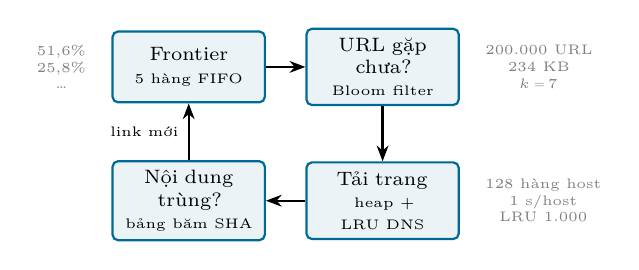
\begin{tikzpicture}[node distance=5mm,font=\scriptsize,
  pbox/.append style={text width=17mm,minimum height=9mm},
  nt/.style={font=\tiny,gray,align=center}]
  \node[pbox] (f) {Frontier\\\tiny 5 hàng FIFO};
  \node[pbox,right=of f] (l) {URL gặp chưa?\\\tiny Bloom filter};
  \node[pbox,below=7mm of l] (t) {Tải trang\\\tiny heap + LRU DNS};
  \node[pbox,left=of t] (x) {Nội dung trùng?\\\tiny bảng băm SHA};
  \draw[parr] (f)--(l);
  \draw[parr] (l)--(t);
  \draw[parr] (t)--(x);
  \draw[parr] (x)--node[left,font=\tiny]{link mới} (f);
  \node[nt,right=2mm of l] {200.000 URL\\234 KB\\$k=7$};
  \node[nt,right=2mm of t] {128 hàng host\\1 s/host\\LRU 1.000};
  \node[nt,left=2mm of f] {51,6\%\\25,8\%\\\dots};
\end{tikzpicture}
\caption{Dòng dữ liệu của crawler. Ghi chú nhỏ là số liệu thật của đồ án ở mỗi bước.}
\label{fig:crawlloop}
\end{figure}

\dsa{Nhiều hàng đợi FIFO theo mức ưu tiên}{FrontQueues}
\vande Trang chủ và trang chuyên mục gần hạt giống cần được tải trước trang sâu mười lớp.

\cu Một hàng đợi duy nhất chỉ biết thứ tự đến trước, không biết trang nào đáng tải. Chọn thẳng mức tốt nhất thì các mức dưới đói vĩnh viễn, vì mỗi trang tải về lại sinh thêm hàng chục URL nông.

\cachgiai Có 5 hàng FIFO, mỗi hàng một mức. Mức của URL là $\ell=\operatorname{clip}(d-[\code{.vn}]-[\text{backlink}\ge5],0,4)$, với $d$ là độ sâu BFS. Bộ chọn bốc ngẫu nhiên theo trọng số $2^{4-i}$, tức $16,8,4,2,1$, và chỉ tính các hàng không rỗng. Hạt giống ngẫu nhiên cố định nên hai lần chạy cho cùng thứ tự.

\vidu Trang \code{.vn} sâu $d=3$ có 5 backlink được mức $3-1-1=1$. Trong 100 lần lấy URL:
\begin{center}\footnotesize
\begin{tabular}{@{}lccccc@{}}
\toprule
Mức & 0 & 1 & 2 & 3 & 4 \\
\midrule
Ưu tiên tuyệt đối & 100 & 0 & 0 & 0 & 0 \\
Bốc theo trọng số & 51,6 & 25,8 & 12,9 & 6,5 & 3,2 \\
\bottomrule
\end{tabular}
\end{center}
Cách thứ nhất không bao giờ chạm tới mức 1 chừng nào mức 0 còn URL. Cách thứ hai ưu tiên mức 0 nhưng mức 4 vẫn được lấy trung bình 3,2 lần.

\dpt Thêm $O(1)$, lấy $O(5)$. Heap theo điểm tốn $O(\log n)$ cho cả hai và vẫn đói.

\dsa{Min-heap theo thời điểm sẵn sàng}{BackQueues, MinHeap}
\vande Crawler có 32 luồng, và quy tắc lịch sự đòi mỗi host cách nhau ít nhất 1 giây. Không kiềm lại thì cả 32 luồng có thể cùng đập vào một trang báo.

\cu Quét mọi host ở mỗi lần lấy URL để tìm host đã hết thời gian chờ, tốn $O(D)$ với $D$ là số host.

\cachgiai Tầng sau có 128 hàng đợi, mỗi hàng chỉ chứa URL của một host \cite{heydon1999mercator}, và bảng băm \code{hostToQueue} ánh xạ host sang hàng. Các hàng nằm trong min-heap theo thời điểm sẵn sàng kế tiếp. Chỉ cần nhìn gốc: gốc chưa tới giờ thì không hàng nào tới giờ. Lấy xong một URL, khóa cộng 1000~ms rồi chèn lại.

Heap cài trên mảng \cite{cormen2009}: con của $i$ ở $2i+1$, $2i+2$. \code{siftUp}, \code{siftDown} dùng ``lỗ trống'': giữ phần tử cần dời trong biến tạm, kéo các phần tử trên đường đi vào lỗ rồi gán một lần, nên mỗi bước 1 phép gán thay vì 3 của \code{swap}. Bất biến: chỉ sửa khóa của một hàng khi nó đang ngoài heap, vì sửa khóa phần tử trong heap làm sai thứ tự mà không báo lỗi.

\vidu Năm host có thời điểm sẵn sàng \code{vne}=100, \code{tt}=250, \code{dt}=400, \code{cafef}=600, \code{zing}=900 ms (Hình~\ref{fig:heap}). Tại $t=100$ ta lấy URL của \code{vne}, đặt khóa $1100$ rồi chèn lại, và gốc mới là \code{tt}=250. Cách quét phải nhìn đủ $D$ host mỗi lần; với 128 hàng là 128 phép so sánh, còn heap chỉ sàng khoảng $\log_2 128=7$ bước.

\begin{figure}[H]
\centering
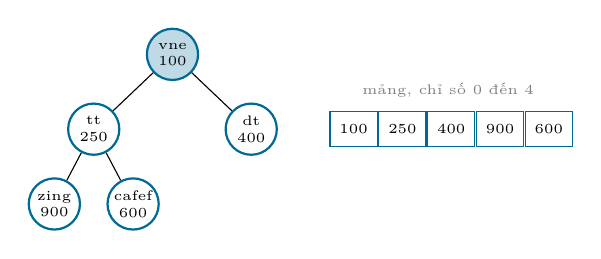
\begin{tikzpicture}[font=\scriptsize,
  hn/.style={circle,draw=linkblue,thick,minimum size=6.5mm,inner sep=0pt,align=center,font=\tiny},
  ac/.style={draw=linkblue,minimum width=6mm,minimum height=4.5mm,inner sep=0pt,font=\tiny}]
\node[hn,fill=linkblue!25] (r) at (0,0) {vne\\100};
\node[hn] (a) at (-1,-0.95) {tt\\250};
\node[hn] (b) at (1,-0.95) {dt\\400};
\node[hn] (c) at (-1.5,-1.9) {zing\\900};
\node[hn] (d) at (-0.5,-1.9) {cafef\\600};
\draw (r)--(a); \draw (r)--(b); \draw (a)--(c); \draw (a)--(d);
\foreach \i/\t in {0/100,1/250,2/400,3/900,4/600}
  \node[ac] at (2.3+\i*0.62,-0.95) {\t};
\node[font=\tiny,gray] at (3.5,-0.45) {mảng, chỉ số 0 đến 4};
\end{tikzpicture}
\caption{Min-heap host theo thời điểm sẵn sàng (ms).}
\label{fig:heap}
\end{figure}

\dpt Xem gốc $O(1)$, chèn và lấy gốc $O(\log n)$, dựng heap bằng Floyd heapify $O(n)$.

\dsa{Bloom filter}{BloomFilter, UrlSeenFilter}
\vande Trang báo liên kết chéo dày đặc nên cùng một URL được rút ra nhiều lần. Cần biết ``URL này gặp rồi chưa'' cho hàng trăm nghìn URL.

\cu \code{HashSet<String>} lưu nguyên chuỗi URL, với 200.000 URL tốn hàng chục MB.

\cachgiai Bloom filter \cite{bloom1970} là mảng $m$ bit (\code{long[]} cùng phép dịch bit) và $k$ hàm băm. Thêm $x$ thì bật $k$ bit $g_i(x)$. Có một bit 0 thì chắc chắn chưa gặp; đủ $k$ bit 1 thì có lẽ đã gặp. Từ số URL dự kiến $n$ và tỉ lệ báo nhầm $p$:
\begin{equation}
m=\Big\lceil-\frac{n\ln p}{(\ln 2)^2}\Big\rceil,\qquad k=\operatorname{round}\Big(\frac{m}{n}\ln 2\Big).
\label{eq:bloom}
\end{equation}
Chỉ hai hàm băm thật được tính (FNV-1a và một hàm đa thức); phần còn lại là $g_i(x)=(h_1(x)+i\,h_2(x))\bmod m$ \cite{kirsch2006}. Báo nhầm ``đã gặp'' chỉ bỏ sót một trang, còn báo nhầm ``chưa gặp'' không xảy ra vì \code{add} chỉ bật bit. Phép \code{bits[i] |= mask} không nguyên tử, nên \code{UrlSeenFilter} bọc ``kiểm tra rồi ghi nhận'' trong \code{synchronized}; thiếu khóa này hai luồng có thể làm mất một phép ghi và sinh ra báo nhầm ``chưa gặp''.

\vidu Với $n=200.000$ và $p=1\%$, công thức cho $m\approx1{,}9$ triệu bit (234~KB) và $k=7$, nhỏ hơn \code{HashSet} cỡ hai bậc độ lớn. Đổi lại, trong 10.000 URL mới khoảng 100 URL bị báo nhầm là đã gặp và bị bỏ qua.

\dpt Thêm và kiểm tra $O(k)$. Bộ nhớ $O(m)$ bit, không phụ thuộc độ dài URL.

\dsa{Bảng băm vân tay nội dung}{ContentSeenFilter}
\vande Hai URL khác nhau vẫn có thể trả về cùng một bài: bài nằm ở hai chuyên mục, bản in, bản AMP, URL kèm tham số theo dõi.

\cu Bloom filter theo URL coi chúng là hai URL lạ nên cho qua cả hai, và kết quả tìm kiếm hiện bài đó nhiều lần.

\cachgiai Đổi thân bài sang chữ thường, gộp khoảng trắng, băm SHA-256 rồi tra trong tập băm. Mỗi trang tốn 64 ký tự hex dù dài bao nhiêu.

\vidu \code{vnexpress.net/bai-1} và \code{vnexpress.net/bai-1.amp} là hai chuỗi khác nhau nên Bloom cho cả hai qua. Thân bài giống nhau sau chuẩn hóa, ra cùng một vân tay 64 ký tự, nên bản thứ hai bị loại. Không có bước này, bài xuất hiện hai lần trong chỉ mục.

\dpt Băm $O(L)$ với văn bản dài $L$, tra tập $O(1)$. Đây là trùng chính xác: khác một ký tự là hai vân tay khác nhau.

\dsa{LRU cache}{LRUCache, DnsResolver}
\vande Mỗi URL cần phân giải tên miền ra IP, mà hàng nghìn URL dùng chung vài host.

\cu Hỏi DNS ở mỗi URL là lãng phí. Bộ nhớ đệm FIFO thì đuổi host vào sớm nhất dù nó đang được dùng liên tục.

\cachgiai Giữ kết quả của 1.000 host dùng gần nhất, đầy thì bỏ host lâu không dùng nhất. Cấu trúc gồm bảng băm (khóa $\to$ nút) và danh sách liên kết đôi tự viết với hai nút lính canh \code{head}, \code{tail}: nút sau \code{head} mới dùng nhất, nút trước \code{tail} sắp bị bỏ. Danh sách phải liên kết đôi để gỡ nút ở giữa trong $O(1)$ mà không duyệt từ đầu. \code{get} cũng dời nút lên đầu, tức là ghi, nên phải lấy khóa ghi.

\vidu Giả sử sức chứa 3 và dãy truy cập \code{vne}, \code{tt}, \code{vne}, \code{dt}, \code{zing}. Sau ba lần đầu danh sách (mới $\to$ cũ) là $[\code{vne},\code{tt}]$ với \code{vne} vừa được dời lên đầu. Thêm \code{dt}, rồi \code{zing} làm đầy và đuổi \code{tt}, host lâu không dùng. FIFO sẽ đuổi \code{vne}, host nóng nhất, buộc phải hỏi DNS lại. Trên 10.000 URL thuộc 5 host, LRU chỉ tra 5 lần thay vì 10.000.

\dpt \code{get}, \code{put} đều $O(1)$. Lớp này dùng lại ở Chương~2 để giữ kết quả tìm kiếm.

\begin{table}[H]
\centering
\caption{Tóm tắt Chương 1.}
\label{tab:c1}
\footnotesize
\begin{tabular}{@{}p{2.0cm}p{3.3cm}l@{}}
\toprule
Cấu trúc & Giải quyết & Chi phí \\
\midrule
Hàng đợi FIFO theo mức & tải trang quan trọng trước, không bỏ đói & $O(1)$ \\
Min-heap & host nào được gửi request tiếp & $O(\log n)$ \\
Bảng băm & host $\to$ hàng đợi & $O(1)$ \\
Bloom filter & URL đã gặp chưa & $O(k)$ \\
Bảng băm SHA-256 & nội dung trùng & $O(L)$ \\
LRU cache & nhớ kết quả DNS & $O(1)$ \\
\bottomrule
\end{tabular}
\end{table}
\subsection*{So sánh các phương án}
Mỗi bài toán của chương có nhiều lời giải đã được dùng thật. Hai bảng dưới liệt kê các cách phổ biến, cách đồ án chọn in đậm và đánh dấu $\checkmark$; $n$ là số phần tử, $D$ số host, $L$ độ dài văn bản, $k$ số hàm băm.

\begin{table*}[!t]
\centering
\caption{So sánh các phương án cho hàng đợi URL và quy tắc lịch sự theo host.}
\label{tab:cmp1a}
\footnotesize
\begin{tabular}{@{}p{1.9cm}p{3.0cm}p{3.0cm}p{3.5cm}p{3.7cm}c@{}}
\toprule
Bài toán & Cách & Chi phí & Ưu & Nhược & Chọn? \\
\midrule
Xếp hàng ưu tiên URL
& Một hàng đợi FIFO & thêm, lấy $O(1)$ & đơn giản nhất, duyệt đúng theo chiều rộng & không biết trang nào đáng tải trước & \\
& Heap ưu tiên theo điểm & thêm, lấy $O(\log n)$ & luôn lấy được URL điểm cao nhất & chậm hơn, mức thấp bị đói vì URL nông sinh ra liên tục & \\
& \textbf{Nhiều hàng FIFO theo mức, bộ chọn có trọng số (kiểu Mercator \cite{heydon1999mercator}): 5 hàng, trọng số $2^{4-i}$} & thêm $O(1)$, lấy $O(5)$ & rẻ, không bỏ đói, mức 0 nhận 51,6\% lượt, tái lập được với hạt giống cố định & chỉ ưu tiên tương đối, mức do heuristic tự đặt & $\checkmark$ \\
\midrule
Lịch sự theo host
& Quét mọi host mỗi lần lấy & $O(D)$ mỗi lần lấy & không cần cấu trúc phụ & 128 phép so sánh mỗi lần, tăng theo số host & \\
& Một \code{sleep} chung giữa hai request & $O(1)$ & một dòng mã & làm chậm cả các host khác nhau, lãng phí 32 luồng & \\
& Hàng đợi theo thời điểm sẵn sàng của từng host, sắp bằng cây cân bằng (\code{TreeMap}) & $O(\log D)$ & có sẵn trong thư viện, duyệt theo thứ tự được & thêm nút đối tượng, hằng số lớn hơn mảng, không tự cài đặt & \\
& \textbf{Min-heap trên mảng, nhìn gốc} \cite{cormen2009} & xem gốc $O(1)$, chèn và lấy $O(\log D)$ & chỉ cần nhìn gốc, bộ nhớ liền, tự cài đặt được & sửa khóa khi đang trong heap làm hỏng thứ tự & $\checkmark$ \\
\bottomrule
\end{tabular}
\end{table*}

\begin{table*}[!t]
\centering
\caption{So sánh các phương án cho URL đã gặp, nội dung trùng và bộ nhớ đệm DNS.}
\label{tab:cmp1b}
\footnotesize
\begin{tabular}{@{}p{1.9cm}p{3.0cm}p{3.0cm}p{3.5cm}p{3.7cm}c@{}}
\toprule
Bài toán & Cách & Chi phí & Ưu & Nhược & Chọn? \\
\midrule
URL đã gặp chưa
& \code{HashSet<String>} & $O(1)$ kỳ vọng; bộ nhớ theo tổng độ dài URL & chính xác, không báo nhầm & 200.000 URL tốn hàng chục MB & \\
& Cơ sở dữ liệu hoặc B-tree trên đĩa & $O(\log n)$ & chính xác, vượt được bộ nhớ, bền vững & mỗi lần kiểm tra là một truy cập đĩa, chậm cho 32 luồng & \\
& \textbf{Bloom filter} \cite{bloom1970,kirsch2006} & $O(k)$; $O(m)$ bit & 234~KB cho 200.000 URL, không báo nhầm ``chưa gặp'' & có báo nhầm ``đã gặp'' (khoảng 1\%), không xóa được & $\checkmark$ \\
& Cuckoo filter & $O(1)$ kỳ vọng & xóa được, thường gọn hơn Bloom khi $p$ nhỏ & chèn có thể phải di chuyển nhiều lần và thất bại khi đầy, cài đặt phức tạp hơn & \\
& Quotient filter & $O(1)$ kỳ vọng & xóa và gộp được, truy cập bộ nhớ liền & cài đặt khó, hiệu năng giảm khi gần đầy & \\
\midrule
Nội dung trùng
& \textbf{SHA-256 chính xác, tra trong tập băm} & băm $O(L)$, tra $O(1)$ & vân tay cố định 64 ký tự hex, loại đúng bản AMP, bản in & khác một ký tự là hai vân tay khác nhau & $\checkmark$ \\
& So sánh nguyên văn từng cặp & $O(nL)$ mỗi trang mới & không sai sót & không dùng được khi $n$ tăng & \\
& SimHash & $O(L)$ tính, so Hamming $O(1)$ trên 64 bit & bắt cả gần trùng (bài sửa vài chữ) & cần ngưỡng khoảng cách và chỉ mục tìm gần đúng, có thể loại nhầm & \\
& MinHash với LSH & $O(L\cdot h)$ cho $h$ hàm băm & ước lượng được độ giống Jaccard & chữ ký lớn hơn, phải chọn $h$ và dải băm & \\
\midrule
Bộ nhớ đệm DNS
& Không đệm & một lần tra mỗi URL & không cần trạng thái & 10.000 lần tra cho 5 host & \\
& FIFO & $O(1)$ & rất đơn giản & đuổi host nóng nhất nếu nó vào sớm & \\
& TTL & $O(1)$ cộng việc quét hạn & khớp với hạn hiệu lực thật của bản ghi & không giới hạn kích thước, phải có thêm cách đuổi & \\
& LFU & $O(1)$ nếu cài kỹ & giữ host dùng nhiều lâu dài & host từng nóng nhưng đã nguội chiếm chỗ mãi & \\
& ARC & $O(1)$ & tự cân bằng giữa mới dùng và dùng nhiều & bốn danh sách, cài đặt phức tạp & \\
& \textbf{LRU: bảng băm cùng danh sách liên kết đôi} & \code{get}, \code{put} $O(1)$ & đơn giản, tự cài đặt đủ, dùng lại ở Chương~2 & một lượt quét lớn có thể đẩy host nóng ra & $\checkmark$ \\
\bottomrule
\end{tabular}
\end{table*}

\textit{Xếp hàng ưu tiên.} Với 5.000 trang, hàng đợi FIFO đơn cũng chạy được, nhưng nó tải theo thứ tự gặp chứ không theo độ quan trọng. Heap theo điểm đúng hơn về ý nghĩa mà đói các mức dưới, vì mỗi trang tải về sinh thêm nhiều URL nông. Năm hàng FIFO với trọng số $2^{4-i}$ giữ chi phí $O(1)$ và cho mức 4 vẫn nhận 3,2 lần trong 100. Khi có tín hiệu tốt hơn độ sâu và backlink, chẳng hạn điểm liên kết tính ngoại tuyến, heap theo điểm đáng dùng hơn.

\textit{Lịch sự theo host.} Cả ba cách đều sửa được lỗi dồn request vào một host, nhưng quét toàn bộ tốn $O(D)$ và \code{sleep} chung làm mất tính song song của 32 luồng. \code{TreeMap} và min-heap cùng $O(\log D)$; heap thắng vì chỉ cần gốc, nằm trên mảng, và cho phép môn học đo trực tiếp \code{siftUp}, \code{siftDown}. Ở quy mô 128 hàng khác biệt thời gian là không đáng kể, nên lý do chọn là sự rõ ràng của cấu trúc.

\textit{URL đã gặp.} \code{HashSet} chính xác và đủ dùng ở 200.000 URL nếu máy có vài chục MB trống, nhưng Bloom filter chỉ cần 234~KB và đây là cách duy nhất ở đây có thể giải thích bằng công thức \eqref{eq:bloom}. Cái giá là khoảng 1\% báo nhầm ``đã gặp'', chỉ làm bỏ sót vài trang. Nếu cần xóa URL (ví dụ để tải lại trang đã đổi), Bloom filter không làm được, và Cuckoo filter hay quotient filter là lựa chọn đúng. Khi tập URL vượt bộ nhớ, B-tree hoặc cơ sở dữ liệu thành bắt buộc.

\textit{Nội dung trùng.} Cái cần loại ở đây là bản AMP, bản in, URL kèm tham số theo dõi: thân bài giống hệt sau chuẩn hóa, nên SHA-256 chính xác đủ và tra $O(1)$. SimHash chỉ đáng dùng khi muốn bắt cả bài đăng lại có sửa vài chữ; khi đó phải thêm chỉ mục tìm theo khoảng cách Hamming và chấp nhận loại nhầm. Đồ án không đo tỉ lệ gần trùng trên 5.000 trang nên không có cơ sở để trả giá đó.

\textit{Bộ nhớ đệm DNS.} Truy cập DNS tập trung vào vài host nóng, đúng kiểu LRU xử lý tốt: 10.000 URL thuộc 5 host chỉ tốn 5 lần tra. LFU hay ARC chỉ tốt hơn khi mẫu truy cập thay đổi theo thời gian hoặc có quét dài, điều chưa xảy ra với dung lượng 1.000 host. TTL không thay thế được LRU mà bổ sung cho nó: nếu chạy lâu ngày, bản ghi DNS hết hạn và cần thêm kiểm tra thời gian.
\section{Chỉ mục đảo và truy vấn}
\label{sec:index}
Chương này biến trang đã tải thành chỉ mục rồi dùng chỉ mục để tìm tài liệu khớp truy vấn. Trang và truy vấn phải được cắt thành từ theo cùng một cách, nếu không thì trang cho ra \code{máy\_tính} còn truy vấn cho ra \code{máy} + \code{tính} sẽ không bao giờ khớp.

\begin{figure}[H]
\centering
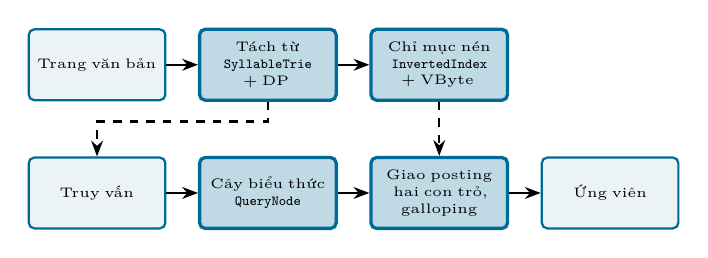
\begin{tikzpicture}[font=\scriptsize,node distance=4mm,
  b/.style={pbox,text width=15mm,minimum height=9mm,font=\tiny},
  bm/.style={pmine,text width=15mm,minimum height=9mm,font=\tiny}]
\node[b] (a1) {Trang văn bản};
\node[bm,right=of a1] (a2) {Tách từ\\\code{SyllableTrie}\\+ DP};
\node[bm,right=of a2] (a3) {Chỉ mục nén\\\code{InvertedIndex}\\+ VByte};
\node[b,below=7mm of a1] (b1) {Truy vấn};
\node[bm,right=of b1] (b2) {Cây biểu thức\\\code{QueryNode}};
\node[bm,right=of b2] (b3) {Giao posting\\hai con trỏ,\\galloping};
\node[b,right=of b3] (b4) {Ứng viên};
\draw[parr] (a1)--(a2); \draw[parr] (a2)--(a3);
\draw[parr] (b1)--(b2); \draw[parr] (b2)--(b3); \draw[parr] (b3)--(b4);
\draw[parr,dashed] (a3.south) -- ++(0,-3.5mm) -| (b3.north);
\draw[parr,dashed] (a2.south) -- ++(0,-2.5mm) -| (b1.north);
\end{tikzpicture}
\caption{Dòng dữ liệu của Chương 2. Hàng trên dựng chỉ mục, hàng dưới trả lời truy vấn. Truy vấn cũng đi qua bộ tách từ ở hàng trên.}
\label{fig:pipe2}
\end{figure}

\dsa{Trie theo âm tiết}{SyllableTrie}
\vande Bộ tách từ liên tục hỏi dãy âm tiết $s_i\dots s_j$ có phải một từ trong từ điển không.

\cu Ghép âm tiết thành chuỗi rồi tra \code{HashSet}. Mỗi vị trí sinh ba chuỗi tạm rồi bỏ, khoảng 15 triệu lần cấp phát trên 5 triệu âm tiết của kho.

\cachgiai Trie mà mỗi cạnh là một âm tiết, đi từ nút hiện tại theo âm tiết kế tiếp mà không cấp phát gì. Bốn độ dài 1 đến 4 được kiểm tra trong một lượt đi, và gặp nút không có cạnh thì dừng vì không từ nào dài hơn bắt đầu từ đây. Trie lưu bằng mảng phẳng: nút là một \code{int}, mọi cạnh nằm trong một bảng băm địa chỉ mở với khóa \code{(nútCha << 32) | idÂmTiết}. Với 185.000 từ (khoảng 460.000 nút), cách này tránh 460.000 đối tượng \code{HashMap}.

\vidu Từ điển có \code{nhà}, \code{nhà\_hàng}, \code{hàng}, \code{hàng\_xóm}. Tại vị trí 0 của ``nhà hàng xóm'', trie đi \code{nhà} (là từ), \code{hàng} (là từ \code{nhà\_hàng}), rồi \code{xóm} không có cạnh nên dừng: 3 bước, 0 chuỗi tạm. Cách cũ dựng ba chuỗi (``nhà'', ``nhà hàng'', ``nhà hàng xóm'') chỉ để tra rồi vứt.

\dpt Tìm cạnh con $O(1)$ kỳ vọng; chèn từ $k$ âm tiết $O(k)$.

\dsa{Quy hoạch động tách từ}{MaxWeightSegmenter}
\vande Tiếng Việt dùng dấu cách giữa các âm tiết chứ không giữa các từ, nên phải chọn chỗ cắt.

\cu Tham lam: lấy từ dài nhất ở mỗi vị trí và không quay lại. ``Nhà hàng xóm'' bị tách thành \code{nhà\_hàng} + \code{xóm}, trong khi đúng là \code{nhà} + \code{hàng\_xóm}.

\cachgiai Đặt các đỉnh $0..n$ giữa các âm tiết. Mỗi từ trong từ điển phủ âm tiết $i$ đến $j-1$ là một cạnh $i\to j$ với trọng số tính từ tần suất \cite{coccoctokenizer}. Cần đường đi tổng trọng số lớn nhất trên DAG:
\begin{equation}
\text{best}[j]=\max_{\,j-4\le i<j}\big(\text{best}[i]+w(s_i\dots s_{j-1})\big),\quad \text{best}[0]=0.
\label{eq:dp}
\end{equation}
Các đỉnh đã có thứ tự tô-pô nên một lượt quét trái sang phải là đủ, mảng \code{trace} lưu lựa chọn thắng để lần ngược. Tên riêng không có trong từ điển đi qua cạnh dự phòng trọng số $0{,}5$.

\vidu Hình~\ref{fig:dag} cho ``nhà hàng xóm''. Tham lam đi $0\to2\to3$ được $9{,}59+3{,}46=13{,}05$ và cho kết quả sai. DP so hai đường vào đỉnh 3 và chọn $3{,}69+9{,}44=13{,}13$, đúng cách tách.

\begin{figure}[H]
\centering
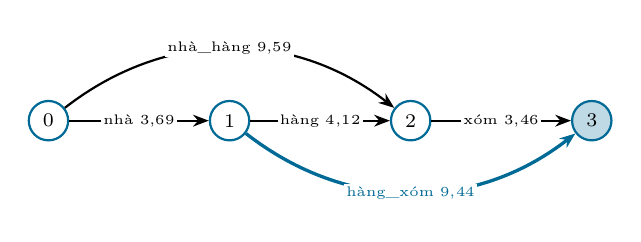
\begin{tikzpicture}[font=\scriptsize,
  nd/.style={circle,draw=linkblue,thick,inner sep=1pt,minimum size=5mm},
  lv/.style={font=\tiny,midway,fill=white,inner sep=0.8pt}]
\node[nd] (n0) at (0,0) {0};
\node[nd] (n1) at (2.3,0) {1};
\node[nd] (n2) at (4.6,0) {2};
\node[nd,fill=linkblue!25] (n3) at (6.9,0) {3};
\draw[parr] (n0)--node[lv]{nhà $3{,}69$} (n1);
\draw[parr] (n1)--node[lv]{hàng $4{,}12$} (n2);
\draw[parr] (n2)--node[lv]{xóm $3{,}46$} (n3);
\draw[parr] (n0) to[bend left=38] node[lv]{nhà\_hàng $9{,}59$} (n2);
\draw[parr,very thick,linkblue] (n1) to[bend right=38] node[lv]{hàng\_xóm $9{,}44$} (n3);
\end{tikzpicture}
\caption{$\text{best}[3]=\max(9{,}59+3{,}46;\ 3{,}69+9{,}44)=13{,}13$. Đường đậm $0\to1\to3$ thắng đường tham lam.}
\label{fig:dag}
\end{figure}

\dpt $O(n)$ cho câu $n$ âm tiết, vì mỗi ô chỉ nhìn lùi tối đa 4 ô.

\dsa{Chỉ mục đảo}{InvertedIndex}
\vande Tìm các trang chứa một từ trong 5.011 trang.

\cu Quét lần lượt cả 5.011 trang cho mỗi truy vấn, chi phí tỉ lệ với kích thước kho.

\cachgiai Bảng băm \code{term} $\to$ posting list, là danh sách các tài liệu chứa term, mỗi phần tử gồm mã tài liệu và các vị trí của term trong đó. Mỗi term được lưu thêm dạng không dấu nên ``may tinh'' vẫn ra ``máy tính''. Posting list luôn tăng dần theo mã tài liệu. Điều này có sẵn mà không cần sắp xếp, vì tài liệu được thêm theo mã tăng dần và chỉ nối vào cuối; lớp ném ngoại lệ nếu bị gọi sai thứ tự. Nhờ đó tra tần suất của term trong một tài liệu là một phép tìm nhị phân.

\vidu Trong Hình~\ref{fig:inverted}, truy vấn \code{hàng\_xóm} tra bảng băm một lần và nhận ngay $[5,31]$, tức 2 tài liệu. Cách quét phải đọc 5.011 trang để ra cùng kết quả.

\begin{figure}[H]
\centering
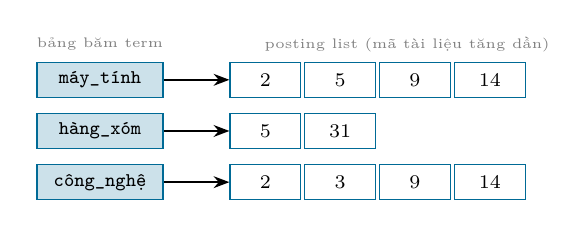
\begin{tikzpicture}[font=\scriptsize,
  cell/.style={draw=linkblue,minimum height=4.5mm,minimum width=9mm,inner sep=1pt},
  term/.style={cell,fill=linkblue!20,minimum width=16mm}]
\node[term] (t1) at (0,0) {\code{máy\_tính}};
\node[term] (t2) at (0,-0.65) {\code{hàng\_xóm}};
\node[term] (t3) at (0,-1.3) {\code{công\_nghệ}};
\foreach \i/\d in {0/2,1/5,2/9,3/14}
  \node[cell] (a\i) at (2.1+\i*0.95,0) {\d};
\foreach \i/\d in {0/5,1/31}
  \node[cell] (b\i) at (2.1+\i*0.95,-0.65) {\d};
\foreach \i/\d in {0/2,1/3,2/9,3/14}
  \node[cell] (c\i) at (2.1+\i*0.95,-1.3) {\d};
\draw[parr] (t1)--(a0); \draw[parr] (t2)--(b0); \draw[parr] (t3)--(c0);
\node[font=\tiny,gray] at (0,0.45) {bảng băm term};
\node[font=\tiny,gray] at (3.9,0.45) {posting list (mã tài liệu tăng dần)};
\end{tikzpicture}
\caption{Chỉ mục đảo.}
\label{fig:inverted}
\end{figure}

\dpt Thêm tài liệu $L$ token $O(L)$; lấy posting list $O(1)$; tra tần suất $O(\log n)$.

\dsa{Kho chuỗi dùng chung (Flyweight)}{TermDictionary}
\vande Kho có 136.768 term phân biệt, nhưng mỗi lần gặp một term bộ tách từ lại tạo một \code{String} mới.

\cu Giữ nguyên các chuỗi đó: khoảng 7 triệu đối tượng, phần lớn là bản sao của nhau.

\cachgiai Một bảng băm ánh xạ nội dung chuỗi sang đúng một bản. Gặp chuỗi đã có thì trả về bản cũ và bản mới thành rác, nên bộ nhớ chuỗi tỉ lệ với số term phân biệt thay vì số lần xuất hiện.

\vidu Nếu \code{máy\_tính} xuất hiện 1.000 lần, cách cũ giữ 1.000 \code{String} còn Flyweight giữ 1. Cộng trên cả kho, 7 triệu đối tượng còn 136.768.

\dpt $O(L)$ mỗi lần tra (băm chuỗi dài $L$).

\dsa{Nén posting list: delta và VByte}{VByteCodec, CompressedPostings}
\vande Chỉ mục phải đủ nhỏ để giữ trong bộ nhớ.

\cu Lưu mỗi mã tài liệu bằng một \code{int} 4 byte làm chỉ mục to 28,1~MB.

\cachgiai Hai bước. Delta: vì danh sách đã sắp, lưu hiệu giữa hai phần tử liền nhau thay cho giá trị. VByte: ghi mỗi số bằng ít byte nhất, 7 bit dữ liệu mỗi byte, bit cao bằng 1 nếu còn byte sau, nên số dưới 128 tốn 1 byte. Trường tần suất được bỏ vì luôn bằng số vị trí. Số vị trí của từng posting không tăng dần, nên được đổi thành tổng tích lũy để dùng chung một bộ mã: $[3,1,2,5]\to[0,3,4,6,11]$.

\vidu Danh sách $[3,17,19,40]$ thành $[3,14,2,21]$, bốn số đều dưới 128 nên mỗi số 1 byte, tổng 4 byte thay cho 16 byte của \code{int}. Số $300=2\cdot128+44$ ghi thành hai byte \code{0xAC 0x02}, trong khi \code{int} luôn tốn 4. Term \code{công\_nghệ} có 1.639 tài liệu trên 5.011, khoảng cách trung bình chừng 3, nên mỗi mã chỉ tốn 1 byte. Trên cả kho, chỉ mục giảm từ 28,1~MB xuống 7,0~MB (còn 25\%).

\dpt Mã hóa và giải mã $O(\text{số byte})$. Mỗi term nén riêng nên truy vấn chỉ giải nén các danh sách nó cần.
\dsa{Cây biểu thức truy vấn}{QueryParser, QueryNode}
\vande Người dùng gõ \code{a b} (AND), \code{a OR b}, \code{-a} (NOT), \code{"cụm từ"} và \code{site:}, nên truy vấn cần một dạng biểu diễn có cấu trúc.

\cu Xem truy vấn như một dãy term rồi giao hết. Cách này không biểu diễn được OR, và nếu tính \code{-a} riêng thì phần bù gần như là cả kho (5.010 trong 5.011 tài liệu với một term hiếm).

\cachgiai Bộ phân tích dựng một cây theo mẫu Composite. Lá là term hoặc cụm từ, nút trong là AND, OR, NOT, và mỗi nút trả về danh sách mã tài liệu đã sắp. Nút NOT không bao giờ được tính một mình: hệ thống tính phần dương trước rồi trừ đi.

\vidu Truy vấn \code{a b -c} với $a=[1,3,5,8]$, $b=[3,5,8,9]$, $c=[5]$ cho cây AND$(a,b,\text{NOT }c)$. Phần dương $a\cap b=[3,5,8]$, trừ $c$ còn $[3,8]$. Cách lấy phần bù của $c$ trước phải dựng một danh sách khoảng 5.010 mã rồi mới giao.

\dpt Phân tích $O(L)$ với $L$ là độ dài truy vấn.

\dsa{Giao và hợp bằng hai con trỏ}{PostingListMerger}
\vande Truy vấn \code{a b} cần các tài liệu có mặt trong cả hai posting list.

\cu Đưa một danh sách vào \code{HashSet} rồi \code{retainAll}. Trên hai danh sách 500.000 phần tử, cách này mất 27~ms vì phải dựng tập và truy cập bộ nhớ rời rạc.

\cachgiai Mỗi danh sách một con trỏ. Hai mã bằng nhau thì ghi lại và tiến cả hai, khác nhau thì tiến con trỏ đang ở mã nhỏ hơn. Phép hợp làm tương tự bước trộn của merge sort. Vì không dựng cấu trúc trung gian và đọc tuần tự, cùng bộ dữ liệu trên chỉ mất khoảng 10~ms.

\vidu $A=[2,5,9,14]$, $B=[3,5,14,20]$.
\begin{center}
\footnotesize
\begin{tabular}{@{}cccl@{}}
\toprule
$A_i$ & $B_j$ & so sánh & hành động \\
\midrule
2 & 3 & $<$ & tiến $A$ \\
5 & 3 & $>$ & tiến $B$ \\
5 & 5 & $=$ & ghi 5, tiến cả hai \\
9 & 14 & $<$ & tiến $A$ \\
14 & 14 & $=$ & ghi 14 \\
\bottomrule
\end{tabular}
\end{center}
Kết quả $[5,14]$ sau 5 lần so sánh, mỗi phần tử được đọc một lần. Cách \code{HashSet} cũng ra $[5,14]$ nhưng phải băm cả 4 phần tử của một danh sách trước.

\dpt $O(m+n)$.

\dsa{Galloping search}{ArrayPostingCursor}
\vande Giao danh sách 5 phần tử với danh sách 4.000 phần tử.

\cu Hai con trỏ vẫn đi qua gần hết danh sách dài, tức khoảng 4.005 bước dù chỉ có 5 ứng viên.

\cachgiai \code{skipTo}$(t)$ tìm phần tử đầu tiên $\ge t$ trong hai pha. Pha một nhảy $1,2,4,8,\dots$ ô cho tới khi vượt $t$. Pha hai tìm nhị phân trong đoạn vừa bao. Nhảy xa $d$ ô tốn $O(\log d)$. Với nhiều term, giao từ danh sách ngắn nhất trước, vì kết quả trung gian chỉ có thể nhỏ đi.

\vidu Danh sách dài có 4.000 mã, mã bằng chỉ số, và ứng viên là $t=3000$. Hai con trỏ bước 3.000 lần. Galloping nhảy $1,2,\dots,2048$ rồi gặp biên (13 lần thăm), sau đó tìm nhị phân trong khoảng $[2048,4000)$ khoảng 11 lần, cộng lại cỡ 24 phép so sánh. Với cả 5 ứng viên, tổng chỉ khoảng 48 bước thay vì 4.005.

Truy vấn cụm từ dùng thêm vị trí. Sau khi giao, mỗi tài liệu được kiểm tra xem có vị trí $p$ sao cho term thứ $i$ nằm ở $p+i$, mỗi lần kiểm tra là một phép tìm nhị phân trên mảng vị trí. Khi phép AND của một truy vấn dài ra rỗng, \code{CandidateResolver} bỏ dần các term ít thông tin nhất rồi giao lại, để người dùng vẫn có kết quả.

\dpt $O(m\log(n/m))$ cho cả phép giao.

\dsa{Trie gợi ý từ khóa}{Trie, SuggestionService}
\vande Người dùng gõ ``hà n'' thì ô tìm kiếm phải gợi ý ngay ``hà nội'' và ``hà nam''.

\cu Quét toàn bộ danh sách từ khóa và so tiền tố từng chuỗi, tốn $O(N\cdot L)$ cho mỗi phím gõ.

\cachgiai Trie theo ký tự, trong đó các chuỗi chung tiền tố đi chung đường. Đi theo tiền tố tới nút của nó, duyệt DFS cây con để gom các từ, rồi lấy $k$ từ phổ biến nhất bằng min-heap cỡ $k$ (xem Chương~3). Mỗi gợi ý được chèn hai lần, có dấu và không dấu, nên gõ ``ha n'' cũng ra. Đọc gợi ý chỉ cần khóa đọc nên nhiều luồng đọc chạy song song được.

\vidu Kho có \code{hà nội} (90 lượt), \code{hà nam} (40), \code{hà giang} (25), \code{hải phòng} (60). Gõ ``hà n'' thì đi 4 ký tự tới nút \code{n}, cây con chỉ có hai từ, trả về \code{hà nội}, \code{hà nam} theo thứ tự lượt. Cách quét phải so cả 4 chuỗi, và trên kho lớn thì so toàn bộ.

\dpt Chèn $O(L)$; gợi ý $O(L+m\log k)$ với $m$ là số từ trong cây con.

\dsa{LRU cache kết quả tìm kiếm}{SearchEngineFacade}
\vande Truy vấn phổ biến được gõ lặp lại nhiều lần.

\cu Chạy lại toàn bộ phân tích, giao danh sách và xếp hạng cho mỗi lần gõ, dù chỉ mục không đổi.

\cachgiai Dùng lại \code{LRUCache} của Chương~1 với sức chứa 200 truy vấn. Cache được tạo lại mỗi khi chỉ mục thay đổi, nên không bao giờ trả kết quả cũ.

\vidu Với sức chứa 2 và chuỗi truy vấn $q_1,q_2,q_1,q_3,q_2$: $q_1$, $q_2$ trượt; $q_1$ trúng; $q_3$ trượt và đẩy $q_2$ ra; $q_2$ trượt lại. Có 1 lần trúng trong 5, lần trúng đó bỏ qua trọn đường truy vấn. Không cache thì cả 5 lần đều chạy đủ.

\dpt $O(1)$ khi trúng cache.

\begin{table}[H]
\centering
\caption{Tóm tắt Chương 2.}
\label{tab:c2}
\footnotesize
\begin{tabular}{@{}p{2.1cm}p{3.2cm}l@{}}
\toprule
Cấu trúc / thuật toán & Giải quyết & Chi phí \\
\midrule
Trie âm tiết & tra từ điển khi tách từ & $O(1)$/bước \\
Quy hoạch động & tách từ đúng & $O(n)$ \\
Chỉ mục đảo & từ $\to$ tài liệu & $O(1)$ \\
Tìm nhị phân & tần suất, vị trí & $O(\log n)$ \\
Flyweight & chuỗi term trùng & $O(L)$ \\
Delta + VByte & chỉ mục quá lớn & $O(\text{byte})$ \\
Cây biểu thức & AND, OR, NOT & $O(L)$ \\
Hai con trỏ & giao, hợp danh sách & $O(m+n)$ \\
Galloping & giao ngắn với dài & $O(m\log\frac{n}{m})$ \\
Trie ký tự & gợi ý từ khóa & $O(L+m\log k)$ \\
LRU cache & truy vấn lặp lại & $O(1)$ \\
\bottomrule
\end{tabular}
\end{table}
\subsection*{So sánh các phương án}
Mỗi bài toán của chương có nhiều cách giải phổ biến. Các bảng dưới đây xếp chúng cạnh nhau theo chi phí, ưu và nhược; cách đồ án chọn được đánh dấu $\checkmark$ và in đậm. Chi phí là độ phức tạp chuẩn hoặc số đã đo ở các mục trên.

\begin{table*}[!t]
\centering
\caption{So sánh các cách tra từ điển và tách từ.}
\label{tab:cmp2a}
\footnotesize
\setlength{\tabcolsep}{3pt}
\begin{tabular}{@{}>{\raggedright\arraybackslash}p{1.9cm}>{\raggedright\arraybackslash}p{3.1cm}>{\raggedright\arraybackslash}p{2.6cm}>{\raggedright\arraybackslash}p{3.9cm}>{\raggedright\arraybackslash}p{4.1cm}c@{}}
\toprule
Bài toán & Cách & Chi phí & Ưu & Nhược & Chọn? \\
\midrule
Tra từ điển khi tách từ
& \code{HashSet} chuỗi ghép & $O(L)$ mỗi lần tra, $L$ là độ dài chuỗi ghép & Ngắn gọn, dùng ngay thư viện chuẩn & Mỗi vị trí sinh chuỗi tạm, khoảng 15 triệu lần cấp phát trên kho 5 triệu âm tiết & \\
& Trie với \code{HashMap} đối tượng ở mỗi nút & $O(1)$ kỳ vọng mỗi bước & Không ghép chuỗi, dừng sớm khi hết cạnh & Mỗi nút một đối tượng, khoảng 460.000 \code{HashMap} cho 185.000 từ & \\
& \textbf{Trie mảng phẳng, bảng băm địa chỉ mở} & $O(1)$ kỳ vọng mỗi bước & Không cấp phát khi tra, ít đối tượng, dễ tự cài đặt & Phải dựng bảng băm đủ lớn; không nén hậu tố chung & $\checkmark$ \\
& Double-array trie & $O(1)$ mỗi bước, hai lần đọc mảng & Tra rất nhanh, bộ nhớ gọn & Dựng và chèn thêm từ phức tạp, chèn có thể phải dời nhiều ô & \\
& DAWG, FST & $O(L)$ theo độ dài khóa & Gộp cả tiền tố lẫn hậu tố chung nên nhỏ nhất & Dựng phức tạp, thường phải dựng từ danh sách đã sắp, khó cập nhật & \\
\midrule
Tách từ tiếng Việt
& Tham lam, lấy từ dài nhất & $O(n)$ & Đơn giản, không cần trọng số & Không quay lại: ``nhà hàng xóm'' thành \code{nhà\_hàng} + \code{xóm} & \\
& Maximum matching hai chiều & $O(n)$, hai lượt quét & Bắt được một số lỗi của một chiều & Vẫn là heuristic; khi hai chiều khác nhau phải thêm luật chọn & \\
& \textbf{Quy hoạch động trọng số} & $O(n)$, mỗi ô nhìn lùi tối đa 4 ô & Tối ưu cả câu theo tổng trọng số; chỉ cần từ điển và tần suất, không cần dữ liệu gán nhãn & Chất lượng phụ thuộc trọng số; từ ngoài từ điển chỉ có cạnh dự phòng & $\checkmark$ \\
& CRF, HMM & Tuyến tính theo độ dài câu, nhân với bình phương số nhãn khi giải mã Viterbi & Học được ngữ cảnh, xử lý tốt từ lạ & Cần kho gán nhãn và bước huấn luyện, mô hình lớn hơn từ điển & \\
& Mô hình nơ-ron (PhoBERT, VnCoreNLP) & Một lượt suy luận qua mạng cho mỗi câu & Độ chính xác tách từ cao nhất trong các cách & Cần dữ liệu huấn luyện, chậm hơn nhiều, phụ thuộc thư viện ngoài, không hợp với bộ tách từ Java tự cài đặt & \\
\bottomrule
\end{tabular}
\end{table*}

\emph{Tra từ điển.} Từ điển có 185.000 từ, nhỏ để nằm trọn trong bộ nhớ, nên điểm nghẽn là cấp phát chứ không phải dung lượng. Trie mảng phẳng bỏ được cả chuỗi tạm lẫn 460.000 đối tượng \code{HashMap} mà vẫn chỉ cần một bảng băm. Double-array nhanh hơn một chút khi tra nhưng phải trả bằng thuật toán dựng phức tạp, không đáng với từ điển nạp một lần. DAWG hoặc FST đáng dùng khi từ điển lên hàng chục triệu mục và dung lượng là ràng buộc chính.

\emph{Tách từ.} Quy hoạch động sửa đúng lỗi của cách tham lam (13,13 so với 13,05 ở ví dụ) mà vẫn $O(n)$ và không cần kho gán nhãn, chỉ cần tần suất từ \cite{coccoctokenizer}. Maximum matching hai chiều rẻ nhưng vẫn là phỏng đoán. CRF và đặc biệt mô hình nơ-ron cho độ chính xác tốt hơn khi có dữ liệu huấn luyện và đủ tài nguyên tính toán; đồ án không có hai thứ đó và bộ tách từ phải chạy nhanh trên 5 triệu âm tiết, nên mức chính xác cao nhất nằm ngoài phạm vi.

\begin{table*}[!t]
\centering
\caption{So sánh cấu trúc chỉ mục và các cách nén posting list.}
\label{tab:cmp2b}
\footnotesize
\setlength{\tabcolsep}{3pt}
\begin{tabular}{@{}>{\raggedright\arraybackslash}p{1.9cm}>{\raggedright\arraybackslash}p{3.1cm}>{\raggedright\arraybackslash}p{2.6cm}>{\raggedright\arraybackslash}p{3.9cm}>{\raggedright\arraybackslash}p{4.1cm}c@{}}
\toprule
Bài toán & Cách & Chi phí & Ưu & Nhược & Chọn? \\
\midrule
Cấu trúc chỉ mục
& Quét tuần tự cả kho & Tỉ lệ với kích thước kho, 5.011 trang mỗi truy vấn & Không tốn bộ nhớ thêm, không cần dựng & Chậm tăng theo kho, không dùng được khi kho lớn & \\
& Ma trận term-document & $O(1)$ mỗi ô; khoảng 685 triệu ô ($136.768\times5.011$) & Tra trực tiếp, dễ viết biểu thức AND, OR & Gần như toàn số 0, quá lớn so với dữ liệu thật & \\
& \textbf{Chỉ mục đảo} & $O(1)$ lấy posting list & Chỉ lưu các ô khác 0, giao danh sách đã sắp rất nhanh & Phải dựng trước; cập nhật chen giữa tốn kém nên đồ án chỉ nối thêm cuối & $\checkmark$ \\
& Suffix array, n-gram index & Tìm chuỗi con $O(m\log n)$ với suffix array & Tìm được chuỗi con bất kỳ, không cần tách từ & Chỉ mục lớn hơn nhiều lần văn bản; không cho sẵn khái niệm từ và posting & \\
\midrule
Nén posting list
& Không nén, \code{int} 4 byte & $O(1)$ mỗi số, 28,1~MB & Nhanh và đơn giản nhất & Tốn nhất, 4 byte cho cả số rất nhỏ & \\
& \textbf{Delta + VByte} & $O(\text{số byte})$, 7,0~MB & Rất ngắn để cài đặt, số nhỏ chỉ 1 byte & Giải mã từng byte có rẽ nhánh; ít gọn hơn các mã đóng gói bit & $\checkmark$ \\
& Simple9, Simple16 & $O(1)$ mỗi từ 32 bit chứa nhiều số & Nén tốt hơn VByte, giải mã nhanh & Phức tạp hơn, giới hạn giá trị tối đa trong mỗi từ & \\
& PForDelta & Khối cố định, giải mã theo vòng lặp phẳng & Rất nhanh, nén tốt trên danh sách dài & Cần khối lớn nên không hợp danh sách ngắn; phải xử lý ngoại lệ riêng & \\
& Elias gamma, delta & $O(\text{số bit})$ & Không cần tham số, gọn khi số nhỏ & Giải mã từng bit, chậm hơn mã theo byte & \\
& Roaring bitmap & AND, OR trên khối $2^{16}$ & Hợp danh sách dày, giao bằng phép bit & Tốn hơn khi danh sách thưa; cài đặt nhiều loại khối & \\
& SIMD-BP128 & Giải mã cả khối 128 số bằng lệnh vector & Nhanh nhất, nén tốt & Cần lệnh SIMD (Vector API hoặc mã gốc), khó cài đặt tay & \\
\bottomrule
\end{tabular}
\end{table*}

\emph{Cấu trúc chỉ mục.} Chỉ mục đảo là lựa chọn mặc định của máy tìm kiếm vì chỉ lưu các cặp (term, tài liệu) thật sự có. Ma trận term-document cần khoảng 685 triệu ô cho kho này, còn quét tuần tự đọc lại 5.011 trang mỗi truy vấn. Suffix array chỉ đáng dùng khi cần khớp chuỗi con bất kỳ, điều mà tìm kiếm theo từ không đòi hỏi.

\emph{Nén posting.} Delta kèm VByte đưa chỉ mục từ 28,1~MB xuống 7,0~MB chỉ bằng vài chục dòng Java, và vẫn giải mã được theo từng term. Ở 5.011 tài liệu, khoảng cách trung bình nhỏ nên VByte đã gần mức nén cần thiết; mức nén thêm không đáng với độ phức tạp. Ở hàng trăm triệu hay hàng tỷ tài liệu thì khác: PForDelta, SIMD-BP128 và Roaring nén tốt hơn và giải mã nhanh hơn rõ rệt, và khi đó chúng là lựa chọn đúng.

\begin{table*}[!t]
\centering
\caption{So sánh các cách giao danh sách, cache kết quả và gợi ý từ khóa.}
\label{tab:cmp2c}
\footnotesize
\setlength{\tabcolsep}{3pt}
\begin{tabular}{@{}>{\raggedright\arraybackslash}p{1.9cm}>{\raggedright\arraybackslash}p{3.1cm}>{\raggedright\arraybackslash}p{2.6cm}>{\raggedright\arraybackslash}p{3.9cm}>{\raggedright\arraybackslash}p{4.1cm}c@{}}
\toprule
Bài toán & Cách & Chi phí & Ưu & Nhược & Chọn? \\
\midrule
Giao danh sách posting
& \code{HashSet} và \code{retainAll} & $O(m+n)$ kỳ vọng; 27~ms trên hai danh sách 500.000 & Ngắn gọn & Dựng tập, truy cập bộ nhớ rời rạc, chậm hơn hai con trỏ & \\
& \textbf{Hai con trỏ} & $O(m+n)$; khoảng 10~ms trên cùng dữ liệu & Đọc tuần tự, không cấu trúc trung gian, cho luôn phép hợp & Đọc cả hai danh sách dù một bên rất ngắn & $\checkmark$ \\
& Tìm nhị phân từng phần tử & $O(m\log n)$ & Tốt khi một danh sách rất ngắn & Không tận dụng vị trí tìm trước đó, kém khi hai danh sách cỡ nhau & \\
& \textbf{Galloping} & $O(m\log(n/m))$ & Thích nghi cả hai trường hợp, nhanh khi lệch kích thước & Cài đặt nhiều bước hơn hai con trỏ & $\checkmark$ \\
& Skip list, skip pointer & $O(m+n/s)$ với bước nhảy $s$ & Nhảy qua đoạn không khớp, hợp danh sách nén theo khối & Tốn thêm bộ nhớ cho con trỏ nhảy; phải chọn $s$ & \\
& Bitmap AND & $O(N/64)$ với $N$ là số tài liệu & Giao và hợp bằng lệnh bit, rất nhanh khi danh sách dày & Kích thước theo $N$ chứ không theo độ dài danh sách, phí với term hiếm & \\
& \textbf{SvS} (ngắn nhất trước) & Kết quả trung gian chỉ nhỏ đi & Giảm công việc cho truy vấn nhiều term & Cần biết độ dài mọi danh sách trước & $\checkmark$ \\
\midrule
Cache kết quả
& \textbf{LRU} & $O(1)$ mỗi lần tra & Đơn giản, thích nghi với truy vấn gần đây & Một loạt truy vấn quét một lần có thể đẩy truy vấn phổ biến ra & $\checkmark$ \\
& LFU & $O(1)$ khi cài đặt cẩn thận & Giữ truy vấn thường xuyên lâu dài & Mục từng phổ biến chiếm chỗ mãi nếu không có cơ chế giảm dần; cài đặt phức tạp hơn & \\
& TTL & $O(1)$ cộng việc dọn mục hết hạn & Dùng được khi dữ liệu đổi mà không biết lúc nào & Phải chọn thời hạn; mục hết hạn có thể còn đúng, mục chưa hết có thể đã cũ & \\
\midrule
Gợi ý từ khóa
& Quét tuyến tính so tiền tố & $O(N\cdot L)$ mỗi phím & Không cần cấu trúc phụ & Chậm tăng theo số từ khóa & \\
& \textbf{Trie ký tự} & Gợi ý $O(L+m\log k)$ & Đi thẳng đến tiền tố, chèn dễ, đọc song song được & Tốn bộ nhớ hơn mảng chuỗi sắp & $\checkmark$ \\
& Ternary search tree, FST & $O(L+\log\sigma)$ hoặc $O(L)$ & Ít bộ nhớ hơn trie; FST nhỏ nhất & Dựng hoặc cập nhật phức tạp hơn & \\
& Chỉ mục n-gram & Tỉ lệ với số n-gram của truy vấn & Khớp được giữa chuỗi và lỗi gõ & Chỉ mục lớn, kết quả cần lọc lại & \\
\bottomrule
\end{tabular}
\end{table*}

\emph{Giao danh sách.} Hai con trỏ cho cùng kết quả với \code{HashSet} nhưng nhanh hơn khoảng 2,7 lần ở phép đo trên, nhờ đọc tuần tự. Khi hai danh sách lệch nhau, galloping chỉ nhảy qua đoạn không cần xét, còn SvS cho phép truy vấn nhiều term bắt đầu từ danh sách ngắn nhất. Bitmap AND sẽ thật sự cạnh tranh ở quy mô này, vì 5.011 tài liệu chỉ cần 79 từ 64 bit, nhưng chỉ mục đã nén theo VByte và phải giải nén rồi dựng bitmap cho mỗi term, nên đồ án giữ danh sách có thứ tự. Skip list đáng dùng khi danh sách nén theo khối và rất dài.

\emph{Cache kết quả.} LRU đủ cho một máy với 200 truy vấn, và vì cache bị tạo lại mỗi khi chỉ mục đổi nên không cần TTL để chống kết quả cũ. LFU có lợi hơn khi phân bố truy vấn lệch mạnh và ổn định trong thời gian dài, điều đồ án chưa có số liệu để khẳng định.

\emph{Gợi ý từ khóa.} Trie ký tự trả lời bằng cách đi theo tiền tố, không phụ thuộc số từ khóa toàn kho. Ternary search tree hoặc FST tiết kiệm bộ nhớ hơn khi danh sách gợi ý lên hàng triệu mục, còn chỉ mục n-gram cần khi muốn gợi ý chịu được lỗi gõ ở giữa từ.
%====================================================================
\section{Xếp hạng}
\label{sec:rank}
%====================================================================
Chương 2 trả về một tập ứng viên. Chương này chấm điểm từng ứng viên, chọn 10 tài liệu tốt nhất và sinh đoạn trích cho chúng.

\begin{figure}[H]
\centering
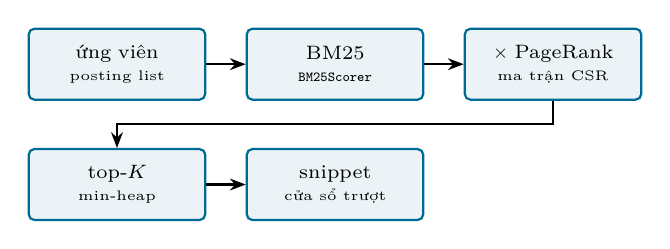
\begin{tikzpicture}[font=\scriptsize,
  rb/.style={pbox,text width=21mm,minimum height=9mm,inner sep=2pt}]
\node[rb] (a) {ứng viên\\{\tiny posting list}};
\node[rb,right=5mm of a] (b) {BM25\\{\tiny \code{BM25Scorer}}};
\node[rb,right=5mm of b] (c) {$\times$ PageRank\\{\tiny ma trận CSR}};
\node[rb,below=6mm of a] (d) {top-$K$\\{\tiny min-heap}};
\node[rb,right=5mm of d] (e) {snippet\\{\tiny cửa sổ trượt}};
\draw[parr] (a)--(b);
\draw[parr] (b)--(c);
\draw[parr] (c.south) |- ++(0,-0.3) -| (d.north);
\draw[parr] (d)--(e);
\end{tikzpicture}
\caption{Luồng dữ liệu của Chương 3.}
\label{fig:pipe3}
\end{figure}

\dsa{Chấm điểm BM25}{BM25Scorer}
\vande Cần một con số cho biết tài liệu liên quan tới truy vấn tới đâu. Số liệu cần thiết đều có sẵn trong chỉ mục: $tf$ là số vị trí trong posting, $df$ là độ dài posting list, độ dài tài liệu được lưu kèm.

\cu Cộng thẳng $tf$ thì tài liệu nhồi từ khóa thắng. Một trang lặp 300 lần từ \emph{hà nội} sẽ có điểm gấp 100 lần trang nhắc 3 lần.

\cachgiai BM25 \cite{robertson2009bm25} cộng điểm từng term trong truy vấn:
\begin{equation}
\text{score}=\sum_{t\in q}\text{idf}_t\cdot
\frac{tf\,(k_1+1)}{tf+k_1\big(1-b+b\,|d|/\overline{|d|}\big)}
\label{eq:bm25}
\end{equation}
với $k_1=1{,}2$, $b=0{,}75$. Phân số không vượt quá $k_1+1$, nên nhồi từ khóa không có lợi. $\text{idf}_t$ chỉ tính một lần cho mỗi truy vấn. TF-IDF là chiến lược thay thế cùng giao diện \code{RelevanceScorer} (mẫu Strategy).

\vidu Hai tài liệu có độ dài bằng trung bình, nên phần tử chuẩn hóa độ dài bằng 1 và phân số còn $2{,}2\,tf/(tf+1{,}2)$.
\begin{center}\footnotesize
\begin{tabular}{@{}lccc@{}}
\toprule
& $tf$ & cộng thẳng $tf$ & phân số BM25 \\
\midrule
Trang bình thường & 3 & 3 & 1,57 \\
Trang nhồi từ khóa & 300 & 300 & 2,19 \\
Tỉ lệ & & 100 lần & 1,4 lần \\
\bottomrule
\end{tabular}
\end{center}
Trang nhồi vẫn nhỉnh hơn một chút, nhưng không còn lấn át.

\dpt $O(c\cdot q\cdot\log d)$ với $c$ ứng viên, $q$ term, và tìm nhị phân $tf$ trong posting list.

\dsa{Ma trận thưa CSR}{SparseMatrix}
\vande PageRank cần ma trận liên kết giữa các trang. Với 5.011 trang chỉ có 239.691 ô khác 0 (0,95\%).

\cu Ma trận đặc \code{double[n][n]} cần $5011^2\times8$ byte $=191{,}5$~MB, gần như toàn số 0.

\cachgiai Chỉ lưu ô khác 0, qua hai chế độ. Khi xây, mỗi hàng là một danh sách kề các cặp (cột, giá trị), vì lúc duyệt liên kết chưa biết trước số phần tử. Xây xong thì \code{freeze()} sang CSR gồm ba mảng phẳng: \code{values[nnz]} (giá trị khác 0, xếp theo hàng), \code{colIdx[nnz]} (cột của từng giá trị) và \code{rowPtr[n+1]} (hàng $i$ nằm ở đoạn $[\text{rowPtr}[i],\text{rowPtr}[i+1])$). Mỗi ô tốn 12 byte thay vì khoảng 32 byte của một đối tượng. Ma trận được lưu sẵn ở dạng chuyển vị, hàng $j$ là các trang trỏ tới $j$, nên phép nhân ra luôn $M^{T}\cdot PR$.

\vidu Đồ thị 4 trang ở Hình~\ref{fig:prgraph} có 5 liên kết. Ma trận chuyển vị đặc có 16 ô, CSR chỉ giữ 5:
\begin{center}\footnotesize
\begin{tabular}{@{}ll@{}}
\code{values} & [1, 0,5, 0,5, 1, 1] \\
\code{colIdx} & [C, A, A, B, D] \\
\code{rowPtr} & [0, 1, 2, 5, 5] \\
\end{tabular}
\end{center}
Hàng C nằm ở đoạn $[2,5)$, tức A, B, D trỏ tới C với trọng số 0,5, 1 và 1. Hàng D rỗng ($5,5$). Với dữ liệu thật, 239.691 ô $\times$ 12 byte $\approx 2{,}9$~MB thay cho 191,5~MB, và chỉ 3 mảng thay vì 239.691 đối tượng.

\dpt Thêm ô $O(1)$ khấu hao; \code{freeze} $O(\text{nnz})$; nhân ma trận với vector $O(\text{nnz})$.

\dsa{PageRank bằng lặp lũy thừa}{PageRankService}
\vande Trang được nhiều trang uy tín trỏ tới nên được đẩy lên cao, nhưng điểm của mỗi trang lại phụ thuộc điểm các trang khác.

\cu Đếm số liên kết vào coi mọi liên kết như nhau, nên một liên kết từ trang rác bằng một liên kết từ trang uy tín.

\cachgiai Công thức tự tham chiếu \cite{brin1998} được giải bằng cách lặp. Bắt đầu với $PR=1/n$ cho mọi trang, mỗi vòng nhân ma trận CSR với vector điểm:
\begin{equation}
PR(j)=\frac{1-\delta}{n}+\delta\Big(\sum_{i\to j}\frac{PR(i)}{\text{out}(i)}+\frac{\text{dangling}}{n}\Big),
\label{eq:pagerank}
\end{equation}
với $\delta=0{,}85$. Điểm của các trang không có liên kết ra (dangling) chia đều cho mọi trang, để tổng luôn bằng 1. Dừng khi tổng thay đổi nhỏ hơn $10^{-6}$ hoặc sau 100 vòng.

\vidu Đồ thị ở Hình~\ref{fig:prgraph}: C nhận 3 liên kết, A chỉ nhận 1. Đếm liên kết vào cho C gấp 3 lần A. Sau 28 vòng lặp, $A=0{,}373$ và $C=0{,}394$, gần bằng nhau vì liên kết duy nhất vào A đến từ C, một trang có điểm cao.

\begin{figure}[H]
\centering
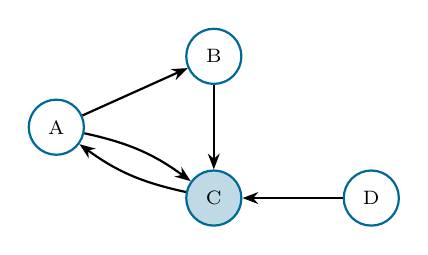
\begin{tikzpicture}[font=\scriptsize,
  nd/.style={circle,draw=linkblue,thick,minimum size=7mm,inner sep=0pt}]
\node[nd] (A) at (0,0) {A};
\node[nd] (B) at (2,0.9) {B};
\node[nd,fill=linkblue!25] (C) at (2,-0.9) {C};
\node[nd] (D) at (4,-0.9) {D};
\draw[parr] (A)--(B);
\draw[parr] (A) to[bend left=12] (C);
\draw[parr] (B)--(C);
\draw[parr] (C) to[bend left=12] (A);
\draw[parr] (D)--(C);
\end{tikzpicture}
\caption{Sau 28 vòng: $A=0{,}373$, $B=0{,}196$, $C=0{,}394$, $D=0{,}038$.}
\label{fig:prgraph}
\end{figure}

\dpt $O(\text{số vòng}\times(\text{nnz}+n))$. Ở đây khoảng 53 vòng trên cùng một ma trận, nên đổi sang CSR một lần là có lợi.

\dsa{Ghép điểm bằng Decorator}{PageRankBoostScorer}
\vande Cần kết hợp điểm liên quan với PageRank thành một điểm cuối.

\cu Công thức cộng $0{,}6s+0{,}3PR$ hỏng vì hai đại lượng khác thang đo: điểm liên quan trung bình $0{,}178$ còn PageRank trung bình $0{,}00035$, nên PageRank chỉ đóng góp 0,1\%.

\cachgiai Nhân điểm liên quan với hệ số tăng: $s'=s\,(1+0{,}3\,\widehat{PR})(1+0{,}1\,\rho)$, với $\widehat{PR}\in[0,1]$ là PageRank đã ép bằng logarit và $\rho$ là tỉ lệ âm tiết truy vấn có trong tiêu đề. Mỗi hệ số là một lớp bọc quanh \code{RelevanceScorer}, nên bật tắt từng tín hiệu được.

\vidu Hai tài liệu giả định, $\rho=0$. Tài liệu X có $s=0{,}20$, $PR=0{,}0004$, $\widehat{PR}=0{,}1$. Tài liệu Y có $s=0{,}18$, $PR=0{,}0100$, $\widehat{PR}=1$.
\begin{center}\footnotesize
\begin{tabular}{@{}lcc@{}}
\toprule
& X & Y \\
\midrule
Cộng: $0{,}6s+0{,}3PR$ & 0,1201 & 0,1110 \\
Nhân: $s(1+0{,}3\widehat{PR})$ & 0,206 & 0,234 \\
\bottomrule
\end{tabular}
\end{center}
Y có PageRank gấp 25 lần mà cách cộng vẫn xếp sau X, vì PageRank chỉ thêm $0{,}003$. Cách nhân đưa Y lên đầu.

\dpt $O(1)$ mỗi ứng viên.

\dsa{Top-$K$ bằng min-heap}{MinHeap.topK, ResultRanker}
\vande Có tới 30.000 ứng viên nhưng chỉ hiển thị 10.

\cu Sắp xếp toàn bộ tốn $O(n\log n)$, khoảng $4{,}5\times10^5$ phép so sánh, để rồi bỏ đi 29.990 phần tử.

\cachgiai Giữ một min-heap cỡ $K$. Gốc là ứng viên yếu nhất trong top hiện tại, cũng là ngưỡng để lọt vào top. Ứng viên mới có điểm cao hơn gốc thì thay gốc rồi \code{siftDown}; thấp hơn thì bỏ qua. Cuối cùng lấy hết $K$ phần tử ra và đảo thứ tự.

\vidu Top-3, heap đã chứa 7,1; 8,4; 9,0. Ứng viên 8,0 lớn hơn gốc 7,1 nên thay gốc rồi \code{siftDown}. Ứng viên 5,2 nhỏ hơn gốc nên bỏ qua sau một phép so sánh. Kết quả 9,0; 8,4; 8,0.

\begin{figure}[H]
\centering
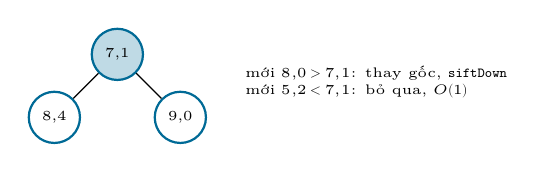
\begin{tikzpicture}[font=\scriptsize,
  hn/.style={circle,draw=linkblue,thick,minimum size=6.5mm,inner sep=0pt,font=\tiny}]
\node[hn,fill=linkblue!25] (r) at (0,0) {7,1};
\node[hn] (a) at (-0.8,-0.8) {8,4};
\node[hn] (b) at (0.8,-0.8) {9,0};
\draw (r)--(a); \draw (r)--(b);
\node[font=\tiny,align=left,anchor=west] at (1.5,-0.35) {mới $8{,}0>7{,}1$: thay gốc, \code{siftDown}\\mới $5{,}2<7{,}1$: bỏ qua, $O(1)$};
\end{tikzpicture}
\caption{Top-3 bằng min-heap. Gốc là ngưỡng để vào top.}
\label{fig:topk}
\end{figure}

\dpt $O(n\log K)$ thời gian, $O(K)$ bộ nhớ. Với $n=30.000$, $K=10$: khoảng $10^5$ phép so sánh so với $4{,}5\times10^5$.

\dsa{Cửa sổ trượt sinh đoạn trích}{SnippetBuilder}
\vande Trong tài liệu $n$ từ, tìm đoạn $w$ từ liên tiếp chứa nhiều từ khóa nhất để hiển thị dưới kết quả. Đây là bước đắt nhất của chương.

\cu Đếm lại từ đầu ở mỗi vị trí tốn $O(n\cdot w)$, và còn làm cho mọi ứng viên: $500\times1.043=521.500$ token.

\cachgiai Đếm từ khóa trong cửa sổ đầu tiên. Mỗi lần dịch cửa sổ một bước, trừ phần tử rời bên trái và cộng phần tử vào bên phải, nên biến đếm luôn bằng số từ khóa trong cửa sổ hiện tại. Chỉ sinh đoạn trích cho $K$ tài liệu đã nằm trong top.

\vidu Tài liệu $n=1.043$ từ, $w=25$.
\begin{center}\footnotesize
\begin{tabular}{@{}lrr@{}}
\toprule
& đếm lại & cửa sổ trượt \\
\midrule
Số bước mỗi tài liệu & 26.075 & 1.068 \\
Số tài liệu xử lý & 500 & 10 \\
Token duyệt & 521.500 & 10.430 \\
\bottomrule
\end{tabular}
\end{center}
Hai thay đổi cộng lại cho kết quả nhanh khoảng 50 lần ở bước đoạn trích.

\dpt $O(n)$ mỗi tài liệu thay vì $O(n\cdot w)$.

\begin{table}[H]
\centering
\caption{Tóm tắt Chương 3.}
\label{tab:c3}
\footnotesize
\begin{tabular}{@{}p{2.0cm}p{3.2cm}l@{}}
\toprule
Cấu trúc / thuật toán & Giải quyết & Chi phí \\
\midrule
BM25 & điểm liên quan, chặn nhồi từ khóa & $O(c\,q\log d)$ \\
Ma trận thưa CSR & ma trận liên kết 191,5~MB & $O(\text{nnz})$ \\
Lặp lũy thừa & tính PageRank & $O(it\cdot(\text{nnz}{+}n))$ \\
Decorator & ghép điểm khác thang & $O(1)$ \\
Min-heap cỡ $K$ & lấy top-10 & $O(n\log K)$ \\
Cửa sổ trượt & đoạn trích tốt nhất & $O(n)$ \\
\bottomrule
\end{tabular}
\end{table}

\subsection*{So sánh các phương án}
Mỗi bài toán của chương có nhiều cách giải phổ biến. Hai bảng dưới đây đặt chúng cạnh nhau theo chi phí, ưu và nhược; cách đồ án chọn được đánh dấu $\checkmark$ và in đậm. Chi phí là độ phức tạp chuẩn, với $c$ ứng viên, $q$ term, $d$ độ dài posting list, $n$ phần tử, $w$ độ rộng cửa sổ.

\begin{table*}[!t]
\centering
\caption{So sánh các phương án: chấm điểm liên quan, biểu diễn ma trận liên kết, tính PageRank.}
\label{tab:c3cmp1}
\footnotesize
\setlength{\tabcolsep}{3pt}
\begin{tabular}{@{}p{1.7cm}p{2.7cm}p{2.6cm}p{4.3cm}p{4.7cm}p{0.8cm}@{}}
\toprule
Bài toán & Cách & Chi phí & Ưu & Nhược & Chọn? \\
\midrule
Chấm điểm liên quan
 & Đếm khớp / boolean & $O(c\,q)$ & Rất đơn giản, không cần thống kê toàn tập & Chỉ lọc có/không, nhồi từ khóa thắng, không xếp hạng được & \\
 & TF-IDF & $O(c\,q)$ & Có trọng số hiếm của term, dễ cài & $tf$ tăng tuyến tính nên bị nhồi từ khóa, chuẩn hóa độ dài yếu & \\
 & \textbf{BM25} \cite{robertson2009bm25} & $O(c\,q\log d)$ & $tf$ bão hòa, chuẩn hóa độ dài, không cần dữ liệu nhãn, chỉ dùng số liệu có sẵn trong chỉ mục & Hai tham số $k_1,b$ chọn tay; không hiểu đồng nghĩa & $\checkmark$ \\
 & BM25F & $O(c\,q\,f\log d)$ với $f$ trường & Tính riêng tiêu đề, nội dung, anchor với trọng số khác nhau & Cần lưu $tf$ theo từng trường và chỉnh trọng số trường & \\
 & Mô hình ngôn ngữ Dirichlet & $O(c\,q\log d)$ & Nền xác suất rõ ràng, làm mượt tự nhiên & Cần xác suất nền của term trên toàn tập và tham số $\mu$; chất lượng thường gần BM25 & \\
 & Learning to rank (LambdaMART) & Suy luận $O(c\cdot T\cdot h)$ với $T$ cây, độ sâu $h$ & Ghép được hàng chục đặc trưng, thường cho chất lượng cao & Cần dữ liệu nhãn liên quan và bước huấn luyện, đồ án không có & \\
 & Truy hồi dày (bi-encoder) & Mã hóa tài liệu một lần; tìm lân cận gần đúng trên vector & Khớp theo nghĩa, bắt được từ đồng nghĩa & Cần mô hình nơ-ron đã huấn luyện, GPU để mã hóa, chỉ mục vector và bộ nhớ cho vector & \\
 & Cross-encoder rerank & $c$ lần chạy mạng cho mỗi truy vấn & Thường chính xác nhất ở bước xếp lại & Cần mô hình huấn luyện có nhãn, GPU, độ trễ cao khi $c$ lớn & \\
\midrule
Biểu diễn ma trận liên kết
 & Ma trận đặc \code{double[n][n]} & $O(n^2)$ bộ nhớ, 191,5~MB & Truy cập ô $O(1)$, mã đơn giản nhất & Gần như toàn số 0; phép nhân vector $O(n^2)$ & \\
 & Danh sách kề đối tượng & $O(\text{nnz})$, khoảng 32 byte/ô & Thêm cạnh dễ, hợp với lúc xây đồ thị & Mỗi ô một đối tượng, tốn bộ nhớ và kém cục bộ cache & \\
 & COO (hàng, cột, giá trị) & $O(\text{nnz})$, 16 byte/ô & Gọn, thêm phần tử đơn giản & Không có chỉ mục hàng, nhân vector phải quét hết và ghi rải rác & \\
 & \textbf{CSR (lưu chuyển vị)} & $O(\text{nnz})$, 12 byte/ô & Ba mảng phẳng, duyệt hàng tuần tự, nhân vector $O(\text{nnz})$ & Khó thêm phần tử sau khi đóng băng, phải xây qua danh sách trung gian & $\checkmark$ \\
 & CSC & $O(\text{nnz})$, 12 byte/ô & Duyệt theo cột nhanh & Cho $M^{T}\!\cdot PR$ cần chuyển vị hoặc ghi rải rác; CSC của $M$ cũng chính là CSR của $M^{T}$ & \\
\midrule
Tính PageRank
 & Giải hệ trực tiếp / nghịch đảo & $O(n^3)$, cần ma trận đặc & Cho nghiệm chính xác một lần & Với $n=5.011$ cỡ $1{,}3\times10^{11}$ phép tính và 191,5~MB; không mở rộng & \\
 & \textbf{Lặp lũy thừa} \cite{brin1998} & $O(\text{số vòng}\cdot(\text{nnz}+n))$ & Chỉ cần phép nhân ma trận thưa với vector, hội tụ được bảo đảm với $\delta<1$ & Hội tụ tuyến tính, số vòng phụ thuộc $\delta$ và ngưỡng dừng & $\checkmark$ \\
 & Gauss-Seidel & $O(\text{nnz}+n)$ mỗi vòng & Dùng ngay giá trị mới, thường cần ít vòng hơn & Kết quả phụ thuộc thứ tự cập nhật, khó song song, xử lý trang dangling phức tạp hơn & \\
 & Monte Carlo (bước đi ngẫu nhiên) & $O(N\cdot L)$ với $N$ bước đi dài $L$ & Cho xấp xỉ rất rẻ, tính được từng phần, dễ cập nhật khi đồ thị đổi & Có sai số ngẫu nhiên, muốn chính xác cao phải đi rất nhiều & \\
 & HITS / TrustRank (hướng khác) & Lặp cỡ $O(\text{nnz})$ mỗi vòng & HITS cho điểm hub và authority theo truy vấn; TrustRank chống spam & Giải bài toán khác: HITS phải tính theo từng truy vấn, TrustRank cần tập hạt giống gán nhãn & \\
\bottomrule
\end{tabular}
\end{table*}

\begin{table*}[!t]
\centering
\caption{So sánh các phương án: ghép tín hiệu điểm, lấy top-$K$, sinh đoạn trích.}
\label{tab:c3cmp2}
\footnotesize
\setlength{\tabcolsep}{3pt}
\begin{tabular}{@{}p{1.7cm}p{2.7cm}p{2.6cm}p{4.3cm}p{4.7cm}p{0.8cm}@{}}
\toprule
Bài toán & Cách & Chi phí & Ưu & Nhược & Chọn? \\
\midrule
Ghép tín hiệu điểm
 & Cộng tuyến tính & $O(1)$ mỗi ứng viên & Dễ hiểu, dễ chỉnh trọng số & Hai đại lượng khác thang nên một bên lấn át (PageRank chỉ góp 0,1\%) nếu không chuẩn hóa & \\
 & \textbf{Nhân hệ số (Decorator)} & $O(1)$ mỗi ứng viên & Không phụ thuộc thang đo, mỗi tín hiệu là một lớp bọc bật tắt được & Trọng số $0{,}3$ và $0{,}1$ đặt tay, cần ép logarit cho PageRank & $\checkmark$ \\
 & Learning to rank & Suy luận $O(c\cdot T\cdot h)$ & Học trọng số tối ưu từ dữ liệu, ghép được nhiều tín hiệu & Cần dữ liệu nhãn và huấn luyện, đồ án không có & \\
 & Reciprocal rank fusion & $O(c\log c)$ cho mỗi danh sách cần sắp & Chỉ dùng thứ hạng nên bỏ qua vấn đề thang đo, không có tham số huấn luyện & Mất độ lớn của điểm; phải sắp riêng từng tín hiệu; hợp hơn khi ghép nhiều bộ truy hồi độc lập & \\
\midrule
Lấy top-$K$
 & Sắp xếp toàn bộ & $O(n\log n)$, $n=30.000$: cỡ $4{,}5\times10^5$ so sánh & Một dòng mã thư viện, kết quả đã có thứ tự & Sắp cả 29.990 phần tử bị bỏ & \\
 & Chọn nhanh (quickselect) & $O(n)$ trung bình, $O(n^2)$ xấu nhất & Tiệm cận tốt hơn, nhanh trên mảng đã có đủ & Cần giữ cả mảng $n$, sửa mảng tại chỗ, vẫn phải sắp $K$ phần tử sau đó & \\
 & \textbf{Min-heap cỡ $K$} \cite{cormen2009} & $O(n\log K)$, bộ nhớ $O(K)$ & Xử lý được dòng dữ liệu, bộ nhớ nhỏ, hầu hết ứng viên bị loại sau một phép so sánh với gốc & Tiệm cận kém quickselect khi $K$ lớn & $\checkmark$ \\
 & Cây thi đấu (tournament tree) & Xây $O(n)$, mỗi lần lấy ra $O(\log n)$ & Lấy lần lượt các phần tử lớn nhất đã có thứ tự & Cần $O(n)$ bộ nhớ phụ cho cây, cài đặt phức tạp hơn & \\
\midrule
Sinh đoạn trích
 & Đếm lại mỗi cửa sổ & $O(n\cdot w)$ & Dễ viết, dễ đúng & Đếm lặp lại cùng các từ, 521.500 token cho 500 ứng viên & \\
 & \textbf{Cửa sổ trượt} & $O(n)$ & Mỗi bước chỉ cộng trừ một phần tử, bộ nhớ $O(1)$ & Đoạn có độ dài cố định nên có thể cắt giữa câu & $\checkmark$ \\
 & Chọn câu theo điểm & $O(n)$ cộng chi phí tách câu & Đoạn trích tròn câu, dễ đọc hơn & Cần tách câu tiếng Việt đáng tin; độ dài đoạn không cố định & \\
 & Mô hình tóm tắt nơ-ron & Một lần suy luận mô hình cho mỗi tài liệu & Văn bản trôi chảy, có thể diễn đạt lại & Cần mô hình huấn luyện, GPU, nếu sinh tự do thì có thể thêm nội dung không có trong trang & \\
\bottomrule
\end{tabular}
\end{table*}

Chấm điểm liên quan. Đồ án có 5.011 trang và không có dữ liệu nhãn, nên mọi hướng cần huấn luyện (LambdaMART, bi-encoder, cross-encoder) đều không dùng được ngay, và hai nhóm nơ-ron còn cần GPU và một chỉ mục vector mà đồ án tự cài bằng Java thì không có. Trong nhóm không cần nhãn, BM25 chỉ dùng $tf$, $df$ và độ dài tài liệu đã nằm sẵn trong chỉ mục, lại chặn được nhồi từ khóa. BM25F đáng dùng khi tiêu đề, anchor và nội dung cần trọng số riêng, nhưng ở đây tiêu đề đã được đưa vào qua hệ số $\rho$. Khi có log truy vấn và nhãn, hoặc cần khớp theo nghĩa, các mô hình nơ-ron và LambdaMART tốt hơn BM25 rõ rệt, và thường được dùng đúng bước xếp lại $c$ ứng viên đầu mà BM25 đã lọc.

Biểu diễn ma trận. Ma trận đặc đơn giản nhất nhưng tốn 191,5~MB cho 0,95\% ô khác 0. Danh sách kề đối tượng gọn hơn, tuy mỗi ô vẫn là một đối tượng. COO và CSR đều cỡ $O(\text{nnz})$, nhưng phép nhân $M^{T}\!\cdot PR$ được thực hiện hàng loạt nên CSR lưu chuyển vị cho truy cập tuần tự, còn COO phải ghi rải rác. CSC chỉ ngang CSR khi lưu cho $M^{T}$, và khi đó nó là cùng một cấu trúc. Nếu ma trận liên tục được thêm cạnh sau khi dựng, hoặc ở quy mô lớn hơn nhiều với nhu cầu cập nhật, COO hay danh sách kề sẽ hợp hơn; đồ án xây một lần rồi chỉ đọc nên CSR phù hợp.

PageRank. Giải trực tiếp cần ma trận đặc và cỡ $n^3$ phép tính, loại ngay với $n=5.011$. Lặp lũy thừa dùng được ma trận CSR có sẵn, mỗi vòng $O(\text{nnz}+n)$, và công thức gốc của \cite{brin1998} là chính nó. Gauss-Seidel thường cần ít vòng hơn và là lựa chọn tốt nếu số vòng trở thành điểm nghẽn, nhưng với khoảng 53 vòng trên ma trận 2,9~MB thì phần lợi không đáng cho độ phức tạp thêm. Monte Carlo trở nên hấp dẫn khi đồ thị lớn đến mức không còn nằm gọn trong bộ nhớ, hay khi cần cập nhật tăng dần. HITS và TrustRank trả lời câu hỏi khác (điểm theo truy vấn, hoặc độ tin cậy từ tập hạt giống) nên không thay thế được điểm uy tín toàn cục ở đây.

Ghép tín hiệu. Cộng tuyến tính hỏng vì thang đo lệch nhau khoảng 500 lần (0,178 so với 0,00035), như ví dụ trong chương. Nhân hệ số trên PageRank đã ép logarit tránh được vấn đề đó mà không cần dữ liệu, và mỗi hệ số là một Decorator tách biệt. Learning to rank sẽ chọn trọng số tốt hơn trọng số đặt tay nếu có nhãn. Reciprocal rank fusion bỏ qua thang đo bằng cách chỉ dùng thứ hạng, hợp với việc trộn kết quả của nhiều bộ truy hồi độc lập; với chỉ hai tín hiệu cùng một tập ứng viên, nó bỏ đi độ lớn của PageRank, vốn là thông tin có ích, và buộc phải sắp riêng từng tín hiệu.

Lấy top-$K$. Với $n=30.000$ và $K=10$, sắp toàn bộ đã đủ nhanh trong thực tế, và quickselect hay cây thi đấu có tiệm cận tốt hơn ($O(n)$ và $O(n+K\log n)$). Min-heap được chọn vì chỉ giữ $K$ phần tử, không cần có sẵn toàn mảng điểm, và đa số ứng viên bị loại bằng một phép so sánh với gốc. Khi $K$ cỡ hàng nghìn hoặc mảng điểm đã nằm trong bộ nhớ, quickselect sẽ nhanh hơn. Đồ án chưa đo sự chênh lệch thời gian giữa các cách này, nên lựa chọn dựa trên độ phức tạp và bộ nhớ chứ không dựa trên số đo.

Sinh đoạn trích. Đếm lại mỗi cửa sổ tốn $O(n\cdot w)$ và lặp công việc, còn cửa sổ trượt chỉ $O(n)$ với một biến đếm, cài được trong vài chục dòng mà không cần thư viện. Chọn câu theo điểm cho đoạn trích đọc tự nhiên hơn vì không cắt giữa câu, và sẽ tốt hơn nếu có bộ tách câu tiếng Việt đáng tin. Mô hình tóm tắt nơ-ron cho văn bản trôi chảy nhất nhưng cần mô hình huấn luyện và GPU, và dạng sinh tự do có thể thêm nội dung trang không có, điều một máy tìm kiếm không nên làm. Vì vậy đồ án giữ cửa sổ trượt và chỉ chạy nó cho $K$ tài liệu đã nằm trong top.

\begin{thebibliography}{99}\footnotesize\itemsep0pt\parskip0pt
\bibitem{heydon1999mercator} A.~Heydon, M.~Najork, Mercator: a scalable, extensible web crawler, World Wide Web 2(4) (1999) 219--229.
\bibitem{bloom1970} B.~H.~Bloom, Space/time trade-offs in hash coding with allowable errors, Commun. ACM 13(7) (1970) 422--426.
\bibitem{kirsch2006} A.~Kirsch, M.~Mitzenmacher, Less hashing, same performance: building a better Bloom filter, in: ESA, 2006, pp.~456--467.
\bibitem{coccoctokenizer} Cốc Cốc, coccoc-tokenizer: a Vietnamese tokenizer, \url{https://github.com/coccoc/coccoc-tokenizer}.
\bibitem{robertson2009bm25} S.~Robertson, H.~Zaragoza, The probabilistic relevance framework: BM25 and beyond, Found. Trends Inf. Retr. 3(4) (2009) 333--389.
\bibitem{brin1998} S.~Brin, L.~Page, The anatomy of a large-scale hypertextual web search engine, Comput. Netw. ISDN Syst. 30(1--7) (1998) 107--117.
\bibitem{cormen2009} T.~H.~Cormen, C.~E.~Leiserson, R.~L.~Rivest, C.~Stein, Introduction to Algorithms, 3rd ed., MIT Press, 2009.
\end{thebibliography}

\end{document}
